\documentclass[twoside,10pt]{book}

\title{RAM-SCB User Manual \\ 
       \hfill \\}

\author{Vania Jordanova, Daniel Welling, Christopher Jeffery\\
       \hfill \\
       {Los Alamos National Laboratory} 
       \hfill \\
       Copyright (c) 2016 
       \hfill \\
       All Rights Reserved}

\makeindex

\input HEADER

\chapter{Introduction \label{chp:intro}}
The \textbf{R}ing current \textbf{A}tmosphere interactions \textbf{M}odel with 
\textbf{S}elf \textbf{C}onsistent magnetic field (\textbf{B}) is a unique code 
that combines a kinetic model of ring current plasma with a three dimensional 
force-balanced model of the terrestrial magnetic field.  The kinetic portion, 
RAM, solves the kinetic equation to yield the bounce-averaged distribution 
function as a function of azimuth, radial distance, energy and pitch angle 
for three ion species ($H^{+}$, $He^{+}$, and $O^{+}$) and, optionally, 
electrons.  The domain is a circle in the Solar-Magnetic (SM) equatorial plane 
with a radial span of 2 to 6.5 $R_{E}$.  It has an energy range of 
approximately 100\,$eV$ to 500\,$KeV$.  The 3-D force balanced magnetic field 
model, SCB, balances the $\textbf{J} \times \textbf{B}$ force with the 
divergence of the general pressure tensor to calculate the magnetic field 
configuration within its domain.  The domain ranges from near the Earth's 
surface, where the field is assumed dipolar, to the shell created by field 
lines passing through the SM equatorial plane at a radial distance of 6.5 
$R_{E}$.  The two codes work in tandem, with RAM providing anisotropic pressure
to SCB and SCB returning the self-consistent magnetic field through which RAM 
plasma is advected.

RAM-SCB has grown from a research-grade code with limited options and static 
magnetic field (RAM) to a rich, highly configurable research and operations 
tool with a multitude of new physics and output products.  This manual provides
a guide to users who want to learn how to install, configure, and execute 
RAM-SCB simulations.  While the code is designed to make these steps as
straight-forward as possible, it is strongly recommended that users review
the publications listed in the Bibliography to ensure a thorough understanding 
of the physics included in the model.  Additionally, all users are asked to 
review the terms of use.

\section{About This Manual}
Users who want to install and begin quickly should start at Chapter 
\ref{chp:quick}, which quickly outlines the path from installation to 
simulation with little detail.  The installation process is discussed fully 
in Chapter \ref{chp:install}.  Instructions on performing simulations, 
as well as several example simulations, are given in Chapter \ref{chp:run}. 
 An outline of using this code in the Space Weather Modeling Framework is 
found in Chapter \ref{chp:swmf}. Useful scripts included in the distribution
are described, in brief, in Chapter \ref{chp:scripts}.
Finally, a complete list of all param file commands is found in Chapter \ref{chp:param}.

\section{TERMS OF USE \& DISTRIBUTION POLICY}

Use of the RAM-SCB software implies agreement with the terms herein.
RAM-SCB is open source software that has been developed at Los Alamos National Laboratory (LANL). The code is based on physics and
numerical methods detailed in the following publications and references therein:

1. Jordanova, V. K. et al. (2006), Kinetic simulations of ring current 
evolution during the Geospace Environment Modeling challenge events, 
J. Geophys, Res., 111, A11S10, doi:10.1029/2006JA011644. \\

2. Zaharia, S. et al. (2006), Self-consistent modeling of magnetic fields 
and plasmas in the inner magnetosphere: Application to the geomagnetic storm,
J. Geophys. Res., 111, A11S14, doi:10.1029/2006JA011619. \\

Redistribution and use in source and binary forms, with or without modification, are permitted provided that the following conditions are met: \\

1. Redistributions of source code must retain the copyright notice, this list of conditions and the following disclaimer. \\

2. Redistributions in binary form must reproduce the copyright notice, this list of conditions and the following disclaimer in the documentation and/or other materials provided with the distribution. \\

3. Neither the name of Los Alamos National Security, LLC, Los Alamos National Laboratory, LANL, the U.S. Government, nor the names of its contributors may be used to endorse or promote products derived from this software without specific prior written permission. \\

This software has been authored by an employee or employees of Los Alamos National Security, LLC,
operator of the Los Alamos National Laboratory (LANL) under Contract No. DE-AC52-06NA25396 with the
U.S. Department of Energy. This software is provided by the copyright holders and contributors "as is" and
any express or implied warranties, including, but not limited to, the implied warranties of merchantability
and fitness for a particular purpose are disclaimed. In no event shall the copyright holder or contributors be
liable for any direct, indirect, incidental, special, exemplary, or consequential damages (including, but not
limited to, procurement of substitute goods or services; loss of use, data, or profits; or business interruption)
however caused and on any theory of liability, whether in contract, strict liability, or tort (including negligence
or otherwise) arising in any way out of the use of this software, even if advised of the possibility of such damage. \\

The references below represent critical development milestones for RAM-SCB. Please consider citing
these works to give the developers proper credit.


\begin{table}[ht]
  \centering
  \begin{tabular}{l|l}
    Citation & Information \\
    \hline
    \hline
    Jordanova et al. [1996] & First description of ring current model (RAM) using dipolar magnetic field \\
    \hline
    Jordanova et al. [2006] & First extension of RAM for non-dipolar magnetic field and coupling with SCB \\
    \hline
    Zaharia et al. [2006] & Description of SCB model and coupling with RAM \\
    \hline
    Jordanova et al. [2010] & Full description of RAM extension for non-dipolar magnetic field \\
    \hline
    Welling et al. [2011] & First full description of one-way coupling with SWMF \\
    \hline
    Welling et al. [2015] & Description of two-way coupling of RAM-SCB
  with SWMF \\
    \hline
  \end{tabular}
\end{table}






\chapter{Quick Start Guide \label{chp:quick}}
This section provides a bare-bones approach for getting started with RAM-SCB. 
The instructions are aimed at users familiar with Unix-like environments.
Tutorial-like guides for each step can be found in other chapters.

\section{Installation}

Installation and compilation of RAM-SCB requires a Fortran compiler, 
Perl interpreter, an MPI library compiled with the preferred Fortran compiler, 
and several external libraries which have 
additional 
requirements (most notably a C compiler, typically standard on Unix-like 
systems.)  The required libraries are:

\begin{enumerate}
\item{\href{http://www.ncl.ucar.edu/Download/}{NCAR's Graphics Library}}

\item{\href{http://w3.pppl.gov/rib/repositories/NTCC/files/pspline.tar.gz}{NTCC's Princeton Spline (Pspline) library}}

\item{\href{http://www.unidata.ucar.edu/downloads/netcdf/ftp/netcdf-4.0.1.tar.gz}{Unidata's NetCDF library}}
\end{enumerate}

If these libraries are installed in non-standard locations, use environment
variables to make them visible to RAM-SCB.  The three variables to be set are
{\tt NCARGDIR}, {\tt PSPLINEDIR}, and {\tt NETCDFDIR}.

Installation of RAM-SCB is handled via the Config.pl script found in the
installation directory.  The {\tt -h} option will print help, but the user 
will almost exclusively use Config.pl as follows:

\begin{verbatim}
Config.pl -install -compiler=pgf90 -mpi=mpich2
\end{verbatim}

Other compiler/MPI combinations are of course available, see Chapter 
\ref{chp:install}.

Finally, use GNU Make to compile and, if desired, test:

\begin{verbatim}
make
make test
\end{verbatim}

\section{Execution}

RAM-SCB is run from \textit{run directories}, create one via {\tt make}:

\begin{verbatim}
make rundir RUNDIR=~/desired_run_location
\end{verbatim}

Run directories are soft-linked to the installation.  This means you can move
them freely and create multiple run directories for simultaneous simulations.
A fresh run directory has everything you need to execute the code immediatetly,
simply start the executable.

\begin{verbatim}
./ram_scb.exe
\end{verbatim}

To customize the simulation, edit the PARAM.in file.  Chapter \ref{chp:param}
has a complete description of all parameters.  Additional input files 
required must be placed in either the {\tt input\_ram} or {\tt input\_scb}
subdirectories; output is located in similarly named locations.

Output data come in two formats: simple ASCII and NetCDF files.  While there
are a plethora of tools available, we recommend users try the Python-based
tools discussed in Chapter \ref{chp:viz}.


\chapter{Installation \label{chp:install}}
Installation and compilation of RAM-SCB requires a Fortran compiler, MPI 
compiled against the chosen Fortran compiler, a Perl interpreter, and several 
external libraries which have additional requirements (most notably a C 
compiler, typically standard on Unix-like systems.)  The configuration is 
done with the Config.pl script; compilation with GNU Make.  The Config/Make 
system follows the tiered makefile standards of the Space Weather Modeling 
Framework (SWMF) project; users of the SWMF should feel right at home using
RAM-SCB.

\section{Installation of Required Libraries}

There are three required libraries that must be installed to use RAM-SCB: 
\href{http://ngwww.ucar.edu/}{NCAR Graphics}, 
\href{http://www.unidata.ucar.edu/software/netcdf/}{Unidata's NetCDF library} 
and \href{http://w3.pppl.gov/ntcc/PSPLINE/}{NTCC's Princeton Spline (Pspline) 
library}. It is possible to find pre-compiled binaries for each library, 
allowing the user to skip the configure, make, and install steps.  However, 
if a binary cannot be found that matches your system and compilers, you will 
be forced to install from source.  Some systems may already have these 
libraries installed; be sure to check before going through unneccessary 
installation work.

\subsection{Installation From Source}
 
Tarballs of the source code can be obtained through these URLs:
\begin{enumerate}
\item{\href{http://www.ncl.ucar.edu/Download/}{http://www.ncl.ucar.edu/Download/} (login required)}

\item{\href{http://w3.pppl.gov/rib/repositories/NTCC/files/pspline.tar.gz}{http://w3.pppl.gov/rib/repositories/NTCC/files/pspline.tar.gz}}

\item{\href{http://www.unidata.ucar.edu/downloads/netcdf/ftp/netcdf-4.0.1.tar.gz}{http://www.unidata.ucar.edu/downloads/netcdf/ftp/netcdf-4.0.1.tar.gz}}
\end{enumerate}


Unpack the tarballs in the usual fashion:
\begin{verbatim}
tar -xzvf netcdf-4.0.1.tar.gz
\end{verbatim}

Because these libraries are not owned or maintained by the authors of RAM-SCB, 
only minimal installation instructions are provided here.  The reader is 
encouraged to explore the websites and help files associated with each package.


\subsubsection{Ncarg Quick Install}
Installation of the NCAR Graphics library from source is an involved process.  
It is strongly suggested that the user first check their system to see if the 
library is already installed or install via binary.

\subsubsection{NetCDF Quick Install}
Unpack the NetCDF tarball, {\tt cd} into the unzipped directory, and use the 
following commands:
\begin{verbatim}
./configure --prefix=/Users/ram_user/netcdf_lib
make install
\end{verbatim}
This will install the NetCDF library in {\tt /Users/ram\_user/netcdf\_lib} 
(the home directory for user \textit{ram\_user}); change the value of 
{\tt --prefix} to select the installation destination.  For installation, 
NetCDF requires only a C compiler.  {\tt gcc} is strongly suggested.

\subsubsection{Pspline Quick Install}
Pspline requires NetCDF, so be sure that NetCDF is correctly installed before 
continuing.  After unpacking the tarball, compile the library using
\begin{verbatim}
make FORTRAN_VARIANT=Portland NETCDF_DIR=~/netcdf_lib
\end{verbatim}
It is important to specify the Fortran compiler that coincides with the 
compiler you will use to make the RAM-SCB executable.  Other options accepted 
by the {\tt FORTRAN\_VARIANT} variable are {\tt PathScale},  {\tt GCC}(gfortran
and g95), {\tt NagWare},  {\tt Fujitsu}, {\tt Intel}, and {\tt Absoft}.  
Ensure that the value of {\tt NETCDF\_DIR} coincides with the installation 
directory of NetCDF.

{\tt make} may fail during the creation of the Pspline test utilities.  If 
this happens, check for the creation of a {\tt lib} directory and several 
\verb*l*.al files contained within.  If they exist, disregard the error 
message and continue to the next step.

Install Pspline as follows (changing the value of {\tt PREFIX} to select 
installation directory):
\begin{verbatim}
make install PREFIX=~/psline_portland
\end{verbatim}
On machines where you will use different compilers, it is helpful to add the 
compiler name to the name of the installation directory.

\subsection{Libraries From Modules}
Well maintained clusters often use the {\tt module} interface for loading
and unloading software packages.  Be sure to explore the available packages
on a new system before going through the arduous task of installing from source!

\begin{verbatim}
module avail
\end{verbatim}
\noindent
will list all available software libraries on the system.  You can load a 
library, unload a library, and list loaded software using the module commands:

\begin{verbatim}
module load package_name
module unload package_name
module list
\end{verbatim}

As an example, here is what you would type on NASA's Pleiades cluster to get
started with RAM-SCB:

\begin{verbatim}
module load comp/intel/10.1.021_64
module load mpi/mpt.1.25
module load netcdf/4.0-i10.1
module load ncarg/4.4.2/intel
module load python/2.6.1
\end{verbatim}

Intel Fortran, MPI, NetCDF and NCAR Graphics are now loaded and ready to use.
Place such commands your shell configuration 
script ({\tt \verb*l~l/.cshrc} or {\tt \verb*l~l/.bashrc} depending on your 
shell) to load modules upon login.  Do not forget to point RAM-SCB to these
libraries as listed below.

\section{Pointing RAM-SCB to External Libraries}
RAM-SCB must be explicitly pointed to libraries installed in non-standard 
places.
There are several ways for RAM-SCB to find the required external libaries, 
summarized in Table \ref{tab:libs}.  The most permanant and convenient method 
is to set an environment variable that RAM-SCB will search for upon 
installation.  They can be set with the following commands:

Bash Shell: {\tt export NETCDFDIR=}\textit{installation path}

C Shell: {\tt setenv NETCDFDIR ``}\textit{installation path}\verb*l''l

Placing these commands into configuration files (e.g. {\tt \verb*l~l/.bashrc} 
or {\tt \verb*l~l/.cshrc}) will load the environment variables at login.  This 
is preferable to typing the commands every session.  Note that the installation
path listed should point to the top level directory for the installation.  
For example, {\tt /Users/ram\_user/ncarg} is sufficient but 
{\tt /Users/ram\_user/ncarg/lib} will cause an error.

Alternatively, it is possible to set the install paths for the external 
libraries using Config.pl during installation.  The use of this method is 
detailed in the next section.  Even if you have set the environment variables, 
using the Config.pl switches will override them.  These switches are 
\emph{only} recognized in conjunction with the {\tt -install} switch 
of Config.pl.

Finally, if you set neither the environment variables or the Config.pl 
switches, the Fortran compiler will look for the libaries in the default 
directories.  This may be useful to test if the libraries are already 
properly installed by the system administrator.  

\emph{If you change the library locations by any method, 
you must reinstall the code.} 

\begin{table}[ht]
  \centering
  \begin{tabular}{l l l}
  \hline\hline
  Library & Environment Variable & Config.pl Switch\\
  \hline
  NCAR Graphics & {\tt NCARGDIR=[...]} & {\tt -ncarg=[...]}\\
  NetCDF & {\tt NETCDFDIR=[...]} & {\tt -netcdf=[...]}\\
  Pspline & {\tt PSPLINEDIR=[...]} & {\tt -psline=[...]}\\
  \end{tabular}
\caption{List of required libraries and methods for expressing their location 
  to RAM-SCB.  Note that the Config.pl switches override environment variables.
  If none are given, the Fortran compiler will search in the default library 
  location.}
\label{tab:libs}
\end{table}

\section{Installation, Configuration, and Compiling \label{subchap:install}}
{\tt Config.pl} handles the installation and configuration of RAM-SCB.  
To view the installation and configuration status, or to view help, use 
the following commands:
\begin{verbatim}
Config.pl
Config.pl -h
\end{verbatim}

To install the code, use the {\tt -install} flag:

\begin{verbatim}
Config.pl -install
\end{verbatim}


Although RAM-SCB will try to use reasonable defaults based on your system, 
there are a number of flags that allow you to customize your installation:
\begin{itemize}
\item{Use {\tt -compiler} to select the Fortran 90 compiler.  
  Common choices include pgf90, ifort, gfortran, and f95(for NAG).}
\item{The {\tt -mpi} flag allows the user to pick which version of MPI to use.
  Choose from mpich, mpich2, Altix, and openmpi.  Alternatively, the 
  {\tt -nompi} flag may be set with no value.  This option is fragile.}
\item{Set {\tt -ncdf} to the path of the NetCDF library installation.  
  If used, this flag overrides the environment variable NETCDFDIR.}
\item{Set {\tt -pspline} to the path of the Pspline library installation.  
  If used, this flag overrides the environment variable PSPLINEDIR.}
\end{itemize}

To exemplify a typical installation, imagine a machine with several different 
Fortran compilers available.  For each compiler available, the user has a 
corresponding installation of Pspline.  The user will use this command to 
properly install RAM-SCB:
\begin{verbatim}
Config.pl -install -compiler=pgf90 -mpi=mpich2 -pspline=~/libs/pspline_portland/
\end{verbatim}

There are other Config.pl options that set up real precision, debug flags, 
and optimization level.  Use {\tt Config.pl -h} to learn about the available 
options.

After the code has been properly configured, compiliation is simple:
\begin{verbatim}
make
\end{verbatim}

Compilation is most likely to fail for two reasons.  The first is RAM-SCB
not finding MPI or another key library.  The second is MPI or an external
library that is installed using a mix of different Fortran compilers.  Be
vigilant when installing each library!

To remove object files before a fresh compilation, use
\begin{verbatim}
make clean
\end{verbatim}

To uninstall RAM-SCB, simply use
\begin{verbatim}
Config.pl -uninstall
\end{verbatim}

\section{Testing the Installation}
Running the RAM-SCB tests is an excellent way to evaluate the success and 
stability of your installation.  To run the tests, simply type
\begin{verbatim}
make test
\end{verbatim}
This will compile RAM-SCB, create a run directory, perform a short simulation 
and compare the results to a reference solution.  If there is a significant 
difference between the test and reference solution, the test will fail.  
Details can be found in \verb*Q*.testQ files in the RAM-SCB directory.  
For a full description of running and interpreting test results, see Chapter 
\ref{chp:test}.

\section{Building Documentation}
To generate a PDF of the latest User Manual, type
\begin{verbatim}
make PDF
\end{verbatim}
The document will be located in the \verb*ldoc/l directory.


\chapter{Testing RAM-SCB \label{chp:test}}
RAM-SCB comes packaged with a test suite to determine if the current 
installation operates correctly and produces the expected results.  
Different tests evaluate different code capabilities and options.  
Testing is an especially powerful development tool for evaluating the impact, 
intentional or not, of changes to the source code.  A summary of the tests
and associated commands can be generated by using {\tt make test\_help}.

\section{Using and Interpreting Test Results}

Tests are called through GNU \verb*lmakel.  To run all available tests, 
simply use the command
\begin{verbatim}
make test
\end{verbatim}
in the RAM-SCB installation directory.  To run a specific test (listed below), 
call that test by name:
\begin{verbatim}
make test1
\end{verbatim}

A test performs the following actions:
\begin{enumerate}
\item{Compile the code with any options required by the particular test.}
\item{Create a run directory entitled \verb*lrun_testl.  If on exists, it will 
  be deleted, so use caution when using this name for any other purpose 
  besides automated testing.}
\item{Copy the required input and parameter files into the new test run 
  directory.}
\item{Run the code.  Test simulations are only long enough to perform the 
  features being tested.}
\item{Perform a specialized version of \verb*ldiffl, included in the 
  distribution, to compare the results produced by the test simulation against 
  reference solutions stored in the output directory of the installation 
  location.  If the two files have values that differ by a certain amount 
  (default is an absolute difference of $10^{-30}$), the test will fail.}
\end{enumerate}

Each of these steps can be called individually by using {\tt make}
\textit{nametest}\_\textit{stepname}, where the step names are {\tt compile},
{\tt rundir}, {\tt run}, and {\tt check}.

If, at any point, the test fails, the details will be recorded in 
\textit{nametest}.diff in the installation directory.  If the test is 
successful, this file will be created but be empty.  Tests that fail at the 
comparitive stage will list all of the differences.  When this happens, 
additional tools to examine the file differences are recommended.  An 
excellent visualization of file differences can be rendered with 
\verb*ltkdiffl, an open source tool that is already installed on many 
Linux machines.

\section{Description of Available Tests}

\subsection{Test 1}

\textbf{Command:} \verb*lmakel \verb*ltest1l

This is the most basic test for RAM-SCB.  It runs RAM-SCB for 300 seconds using
Volland-Stern electric field, constant dipole magnetic field (no SCB 
calculation), and LANL fluxes.  \textbf{SHIELDS-RC} users should rely on this
test.

\subsection{Test 2}

\textbf{Command:} \verb*lmakel \verb*ltest2l

Test 2 repeats the previous test, but stops half way through the simulation,
writes restart files, and restarts the run.  This excercises the code's 
ability to seamlessly restart a simulation at any arbitrary point.

\subsection{Test 3}

\textbf{Command:} \verb*lmakel \verb*ltest3l

Test 3 activates SCB, uses the more complicated Tsyganenko 89 boundary 
conditions and Weimer 2000 empirical electric field.  This is the base test
for SCB functionality and ionosphere-to-equator electric potential mapping.



\chapter{Performing Simulations \label{chp:run}}
%\section{Run Directories \label{subchap:rundir}}
Running RAM-SCB occurs not in the installation directory, but through 
\textit{run directories} -- special directories that keep your simulations 
separate from the installation and other simulations.  To create a run 
directory, simply use the {\tt make} interface:

\begin{verbatim}
make rundir
\end{verbatim}
\noindent
{\tt make} will unpack some default inputs and organize a new directory
aptly named {\tt run}.  Note that if a run directory exists that is called
``run'', RAM-SCB will not over write it and {\tt make} will complain.  

The first thing you should do is rename your run directory and move it to
a place that makes sense given the constraints of your system.  For example,
let's pretend we're using NASA's Pleiades system and doing a set of validation
simulations.  On this system, you typically install code on your home 
directory, but must run from designated directories called ``nobackupXX'' 
(where XX is the number of the directory and nobackup tells you why you 
didn't install your code there.)  From the install directory, make and move
your first run directory:

\begin{verbatim}
make rundir
mv run /nobackup10/username/run_valid
\end{verbatim}
\noindent

Run directories soft link to the installation directory, so as long as you 
don't move, uninstall, or otherwise molest your installion, you can put the
run directory where ever you want.  Furthermore, you are not limited to a single
run directory.  Adding more allows you to run more simulations simultaneously
from a single installation.  Using the {\tt PARAM} interface, described below,
you can perform many very different simulations at once without re-compiling
the code.  Let's add another run directory, but using {\tt make} variable
syntax to make, name, and move the directory in one line:

\begin{verbatim}
make rundir RUNDIR=/nobackup10/username/run_valid2
\end{verbatim}
\noindent
The variable {\tt RUNDIR} sets the location without any extra hassle.  Each
of the two run directories created in this example use the same installation
of RAM-SCB but have different inputs and outputs.  They can be run 
simultaneously without interfering with each other.

Let's look inside a typical run directory:

\begin{figure}[h]
  \begin{center}
    \includegraphics[width=25pc,clip=True,angle=90]{rundir.ps}
  \end{center}
  \caption{Run directory layout.  Gray and green rounded boxes indicate 
  subdirectories; green boxes are directories that are soft linked one level
  up for convenience.  Yellow boxes are key input files, the red box is the
  linked RAM-SCB executable, and other data input files are listed without
  boxes.}
  \label{fig:rundir}
\end{figure}

Figure \ref{fig:rundir} shows the default run directory organization.  The
IM directory is where most input and output occurs; subdirectories shaded
green are soft-linked to the top run level for convenience.  These directories
are self explanatory outside of {\tt output\_swmf}, which is for runs that use
SWMF output in stand-alone mode.  Enough inputs are
given in the input directories for a sample simulation right away.  
The red box in Figure \ref{fig:rundir} denotes the linked executable.  The final
files, denoted as yellow boxes, are the final input files.  {\tt w2k.dat} is
the Weimer 2000 empirical model data file, {\tt omni.txt} is solar wind input 
file from the OMNI database, and {\tt RamIndices.txt} is a list of 
geomagnetic indices.  The necessity of these three files is discussed below.

Finally, there is {\tt PARAM.in}, the run-time configuration file that is used
to tell RAM-SCB what and how it should simulate.  The {\tt PARAM} interface,
identical to the one used by the SWMF, is simple.  Any line of text in the
file not preceeded by a \# symbol is ignored, so comment your file to your
heart's content.    Any text preceeded by \#, however, is a interpreted as
a {\tt PARAM} command.  A generic command takes the form,

\begin{verbatim}
#COMMANDNAME
Parameter1       ParameterName
Parameter2       ParameterName
...
ParameterN       ParameterName
\end{verbatim}

The exact values of the parameters are command specific; the parameter names
are simply tab-delimited from the parameters and are not needed (keeping
them is recommended to keep your file clear and easily understood!)  Here
are a few commands in action:

\begin{verbatim}
#STARTTIME 
2006	iYear 
7	iMonth 
19	iDay 
0	iHour 
0	iMinute 
0	iSecond

#OUTERBOUNDARY 
LANL	NameBoundPlasma 
T89C	NameBoundMag

#VARIABLEDT
T       DoVariableDt

#STOP
-1      MaxIteration
300     tSimulationMax
\end{verbatim}

First, take note that the parameter values can take many forms: rational 
numbers, integers, logical values, or strings of text.  Remember that the
trailing descriptions are not read by RAM-SCB; they are there to help you
remember what each value does.  In order, this list of {\tt PARAM} commands sets
the start date and time of the simulation, sets the plasma and magnetic field
outer boundary conditions, turns on variable timestepping, and tells the
code to run for unlimited iterations but only 300 seconds.  All commands are
described in detail in Chapter \ref{chp:param}.

Once your {\tt PARAM} file is customize, execute RAM-SCB.

\begin{verbatim}
./ram_scb.exe
\end{verbatim}

RAM-SCB will begin; a lot of information will be written to screen that updates
the user of its progress.  Experienced Unix users know all of the tricks to
capture that output; the following copies the output to file while preserving
the output to screen:

\begin{verbatim}
./ram_scb.exe | tee runlog.txt
\end{verbatim}


\section{Required Inputs \label{subchap:input}}

Ring current models have three basic requirements: plasma fluxes at the outer
boundary, magnetic field, and electric field throughout the equatorial plane.
RAM-SCB fulfills these requirements slightly differently than other ring
current models thanks to its sophisticated self-consistent magnetic field.
Electric field may be specified either in the equatorial plane directly or as an
ionospheric potential that is mapped along SCB field lines.  Magnetic field
is supplied as a shell surrounding the SCB domain, which consists of the body
containing all field lines passing through the RAM equatorial domain.  Plasma
fluxes remain a simple specification about the outer boundary of RAM.
In RAM-SCB, there are many ways to specify these; refer to Chapter
\ref{chp:param} for commands that select inputs.

Plasma fluxes can be provided one of two ways: the first is coupling with the
SWMF, covered in Chapter \ref{chp:swmf}.  The second is to use ``GeoMlt'' files,
a product of LANL geosynchronous observations.  These files can be obtained 
on request from the data caretakers; sample files are provided with the 
distribution.  These files come in pairs per day; an ion and electron file
exists for each day for which there is data coverage.  Because the source
observations do not readily differentiate between different ion species, the
$K_{P}$/$F_{10.7}$ dependent empirical relationship of 
\textit{Young et al.,} [1982] is used internally to divide up the 
Hydrogen flux in the input files.  The $K_{P}$ and $F_{10.7}$ indices are 
packaged in the RamIndices.txt input file; the user need not worry about them
for historical simulations.

Convection electric potential can be specified in a plethora of ways.  The 
simplest is to use the $K_{P}$ dependent Volland-Stern electric field.  This
requires no additional input files beyond RamIndices.txt.  The Weimer 2000
empirical model can also be used; like Volland-Stern, it is an internal 
calculation.  Because this model depends on solar wind conditions, users
must supply an input file that contains this data from the OMNI database.
The Weimer 2000 potential is mapped along SCB field lines to the equatorial
plane automatically.  Finally, SWMF electric fields can be used; this is 
covered later.  Though it is possible to supply Weimer 2000 and SWMF potentials
in the equatorial plane without SCB mapping, this approach requires extensive
work by the user as is not recommended.
See the entry on the command \verb*l#EFIELDl for additional details on file
formats and obtaining these inputs.

Magnetic field boundary conditions can be supplied via three sources: a
simple dipole model, from one of the Tsyganenko empirical models, or from the
SWMF.  When using a dipole, it is possible to use a dipole with or without
the SCB calculation.  Tsyganenko 89 (T89) input files are provided with the
distribution and require no additional input from the user.  Input from
more complex Tsyganenko models require substantial work to acquire, they are
not recommended for most users.  See the entry for the \verb*l#OUTERBOUNDARYl
command in Chapter \ref{chp:param} for more details.

All files listed above must be placed in their respective input files in the
run directory.  Other input files required by advanced options (e.g. virtual
satellites) should be placed in the top level of the run directory.  Each
run directory requires its own set of inputs.

\section{Restarting Simulations \label{subchap:restart}}
It is often desirable to split a simulation up into several parts.  For example,
you may want to split a very long simulation up into separate executions, or
change parameters at certain parts of a storm, or perhaps a simulation was 
interrupted undesireably.  Restart files allow you to continue a simulation
seamlessly.

Throughout a simulation, restart files are being written to the {\tt restartOUT}
folder of the run directory.  The files are written at a set frequency and at 
the end of a successful run (both of these options are configuarble through
the {\tt PARAM} interface.)  Only the most recent restart is saved, users
can periodically pull these files out of {\tt restartOUT} if they prefer a 
back log of restarts.  These files contain the full distribution functions as
well as the start time, current time, and current iteration at the point that
the restart was written.

To restart a run, first move restart files from {\tt restartOUT} to 
{\tt restartIN}. Then, either create a new {\tt PARAM.in} file or edit the
existing one such that no \verb*l#STARTTIMEl command is present (remember, the
restart file knows this information already), the run time exceeds the current
time listed in the restart file, and the command \verb*l#RESTARTl is included.
This tells RAM-SCB to restart the simulation rather than start anew.  Restarts
are carefully implemented to preserve files in the output directories and 
continue the simulation as if there was no interruption.

For an example of restarting a simulation, run Test 2 and inspect the 
{\tt PARAM.in} files as well as the contents of {\tt restartIN} and 
{\tt restartOUT}.

\section{Output}
RAM-SCB, by default, has a rich output set.  This can be expanded by activating
other output file types via the {\tt PARAM} interface, be sure to review
the commands listed in Chapter \ref{chp:param}.  Table \ref{tab:out}
summarizes the output that can be generated by RAM-SCB.  Visualization of
these files is covered in Chapter \ref{chp:viz}.


\begin{table}[ht]
  \centering
  \begin{tabular}{l l l l l}
  \hline\hline
   Type & Extension &  Format & Default? & Contents\\
  \hline
  Log file & \verb*q*.logq & ASCII & Yes & Dst, integrated values\\
  Pressure files & \verb*l*.inl & ASCII & Yes & $\perp$ and $\parallel$ partial pressures\\
  Trapped files & \verb*l*.tl & ASCII & Yes & Averaged trapped fluxes\\
  E-Field files & \verb*l*.inl & ASCII & Yes & Equatorial electric potential\\
  Boundary files & \verb*l*.datl & ASCII & Yes & Fluxes at the outer boundary\\
  Full flux files & \verb*l*.ncl & NetCDF & No & Full equatorial flux information\\
  3D flux files & \verb*l*.ncl & NetCDF & No & Fluxes in the full 3D domain\\
  Virtual Satellites &\verb*l*.ncl & NetCDF & No & Satellite specific values\\
  Field integral files &\verb*l*.datl & ASCII & Yes & $h$, $I$ geometric integrals\\
  Magnetic field file &\verb*l*.ncl & NetCDF & No & Full 3D SCB field\\
  Potential file &\verb*l*.ncl & NetCDF & No & Ionospheric and equatorial electric potential\\
  3D pressure file&\verb*l*.ncl & NetCDF & No & Full 3D anisotropic pressure\\ 
  \end{tabular}
\caption{List of available output files.}
\label{tab:out}
\end{table}



\chapter{Output Visualization \label{chp:viz}}
RAM-SCB output can be visualized in a number of different ways depending on
the user's tastes and preferences.  However, a standard library for opening,
manipulating, and plotting exists as a sub-module of Spacepy.  Users may
find this freely available Python library at
\href{http://spacepy.lanl.gov/}{spacepy.lanl.gov}.  Alternatively,
development versions can be obtained via the project's
\href{http://sourceforge.net/projects/spacepy/}{Source Forge} page.  The
RAM-SCB module is nested under {\tt spacepy.pybats.ram}.

Stand-alone code snippets for both Python and Matlab can be found in the
{viz} directories.  These routines are largely out-of-date and not maintained.
We recommend caution when using them.


\chapter{RAM-SCB and SWMF \label{chp:swmf}}
RAM-SCB may be used as a component to the Space Weather Modeling Framework.
Under this mode, RAM-SCB receives initial and boundary conditions from the
Framework's other components and returns plasma properties to create a two-way
coupled system.

%INSERT TABLE OF COUPLING DESCRIPTIONS.

\section{Installing RAM-SCB as a SWMF Component}

Obtain a copy of the SWMF and, if necessary, unpack the tarball.  Descend into
the Inner Magnetosphere (IM) directory of the Framework.  This is where all
inner magnetosphere-type codes used by the Framework are located.  Copy the
entire RAM-SCB directory here as {\tt RAM\_SCB}.  It is important to name the
directory correctly. CVS users should note that checking out RAM-SCB directly into the SWMF directories will be
tricky because of conflicting CVS files located in each Framework directory. Use CVS carefully! 

Next, move or remove the share directory. RAM-SCB will be using the version obtained through the
SWMF. Additionally, making RAM-SCB's share directory unavailable signals RAM-SCB to go into component mode.

Installing the SWMF and RAM-SCB happens concurrently using the Config.pl
script from the top-level directory of the SWMF.  



\chapter{Included Scripts \label{chp:scripts}}
RAM-SCB comes packaged with many helpful scripts that aid the user.  These 
scripts are written either in Perl or Python with the standard libraries only.
This allows them to be run on many systems without needing to install 
additional software as both languages are ubiquitous in Unix-like 
environments.  The subdirectory {\tt Scripts} contains several helpful 
scripts that are unique to RAM-SCB while the subdirectory {\tt Share/Scripts}
contains scripts designed for SWMF-like applications but often useful for 
RAM-SCB as well.

All scripts are designed to be called from the command line and have a common
help feature:
\begin{verbatim}
ScriptName -h
\end{verbatim}
\noindent will print out the script's help text.  This info is typically 
more complete and up-to-date than the info listed here.

While all RAM-SCB scripts are listed here, only a handful of SWMF scripts are
described.  Be sure to explore the {\tt Share/Scripts} directory before you
constructing your own solutions to common problems (e.g. endian conversions, 
PARAM-checking, etc.) 

\section{Config.pl (SWMF Script)}
{\tt Config.pl} is part of the SWMF \textit{Config} system for installing and
pre-configuring RAM-SCB in both stand-alone and component modes.  
Use of {\tt Config.pl} is covered extensively in Chapter \ref{subchap:install}.

\section{DiffNum.pl (SWMF Script)}
{\tt DiffNum.pl} is a powerful, quantitative re-write of the popular {\tt diff}
utility.  It compares two files, finds and quantifies differences in any
numerical entries, and, if any are found, lists the differences and raises an
exception.  The main purpose of {\tt DiffNum.pl} is to find and quantify 
failures in RAM-SCB tests.

Usage:
\begin{verbatim}
DiffNum.pl [options] File1 File2
\end{verbatim}

Common options include {\tt -a=VALUE} and {\tt -r=VALUE}, which allow the user
to ignore absolute and relative differences less than {\tt VALUE} and {\tt -t}
which turns off the comparison of text.


%\section{GetOmni.py (RAM-SCB Script) \label{subchap:getomni}}
%Script forthcoming.

\section{CatLog.py (RAM-SCB Script)}
A common problem in both RAM-SCB and many SWMF modules is many fractured, 
separate log files from a single simulation that required several restarts.
Often, these log files overlap in time because a simulation did not complete
and restarting results in re-simulating a small portion of the run.  
Manually concatenating these log files together into a single seamless, 
monotonic file can be time consuming.

{\tt CatLog.py} concatenates many log files into a single file.  It assumes that
the first column of the log file is either run iteration or run time and uses
this info to check for and remove overlapping entries.

Usage:
\begin{verbatim}
CatLog.py [options] log1 log2 [log3] [log4]...[logN]
\end{verbatim}

Files 2 through N will be appended to the first file.  Unix wild-card 
characters can be used to get file-globbing effects.  If the headers of any
of the trailing log files does not match the leading file, it is discarded.
If the leading file includes a wild-card character, the files are arranged and
appended in alpha-numeric order.  Available options include {\tt -debug}
(print debug information), {\tt -rm} (remove all but first log file), and
{\tt -nocheck} (deactivate checking for overlapping entries.)  See 
{\tt CatLog.py -h} for examples.



% Complete List of Input Commands
\chapter{Complete List of Input Commands \label{chp:param}}

The content of this chapter is generated from the PARAM.XML file.
The XML file can be read with an editor and can be used
for creating PARAM.in files by copying small parts from them.

The transformation of the XML
format into LaTex is done with the share/Scripts/XmlToTex.pl
script. This script generates index terms for all commands,
which are used to create an alphabetical index at the end of this chapter.

\input{RAM_SCBXML}

\newpage
\addcontentsline{toc}{chapter}{{\bf Index of Input Commands}}
% Index for the commands
\documentclass[twoside,10pt]{book}

\title{RAM-SCB User Manual \\ 
       \hfill \\}

\author{Vania Jordanova, Daniel Welling, Christopher Jeffery\\
       \hfill \\
       {Los Alamos National Laboratory} 
       \hfill \\
       Copyright (c) 2016 
       \hfill \\
       All Rights Reserved}

\makeindex

\input HEADER

\chapter{Introduction \label{chp:intro}}
The \textbf{R}ing current \textbf{A}tmosphere interactions \textbf{M}odel with 
\textbf{S}elf \textbf{C}onsistent magnetic field (\textbf{B}) is a unique code 
that combines a kinetic model of ring current plasma with a three dimensional 
force-balanced model of the terrestrial magnetic field.  The kinetic portion, 
RAM, solves the kinetic equation to yield the bounce-averaged distribution 
function as a function of azimuth, radial distance, energy and pitch angle 
for three ion species ($H^{+}$, $He^{+}$, and $O^{+}$) and, optionally, 
electrons.  The domain is a circle in the Solar-Magnetic (SM) equatorial plane 
with a radial span of 2 to 6.5 $R_{E}$.  It has an energy range of 
approximately 100\,$eV$ to 500\,$KeV$.  The 3-D force balanced magnetic field 
model, SCB, balances the $\textbf{J} \times \textbf{B}$ force with the 
divergence of the general pressure tensor to calculate the magnetic field 
configuration within its domain.  The domain ranges from near the Earth's 
surface, where the field is assumed dipolar, to the shell created by field 
lines passing through the SM equatorial plane at a radial distance of 6.5 
$R_{E}$.  The two codes work in tandem, with RAM providing anisotropic pressure
to SCB and SCB returning the self-consistent magnetic field through which RAM 
plasma is advected.

RAM-SCB has grown from a research-grade code with limited options and static 
magnetic field (RAM) to a rich, highly configurable research and operations 
tool with a multitude of new physics and output products.  This manual provides
a guide to users who want to learn how to install, configure, and execute 
RAM-SCB simulations.  While the code is designed to make these steps as
straight-forward as possible, it is strongly recommended that users review
the publications listed in the Bibliography to ensure a thorough understanding 
of the physics included in the model.  Additionally, all users are asked to 
review the terms of use.

\section{About This Manual}
Users who want to install and begin quickly should start at Chapter 
\ref{chp:quick}, which quickly outlines the path from installation to 
simulation with little detail.  The installation process is discussed fully 
in Chapter \ref{chp:install}.  Instructions on performing simulations, 
as well as several example simulations, are given in Chapter \ref{chp:run}. 
 An outline of using this code in the Space Weather Modeling Framework is 
found in Chapter \ref{chp:swmf}. Useful scripts included in the distribution
are described, in brief, in Chapter \ref{chp:scripts}.
Finally, a complete list of all param file commands is found in Chapter \ref{chp:param}.

\section{TERMS OF USE \& DISTRIBUTION POLICY}

Use of the RAM-SCB software implies agreement with the terms herein.
RAM-SCB is open source software that has been developed at Los Alamos National Laboratory (LANL). The code is based on physics and
numerical methods detailed in the following publications and references therein:

1. Jordanova, V. K. et al. (2006), Kinetic simulations of ring current 
evolution during the Geospace Environment Modeling challenge events, 
J. Geophys, Res., 111, A11S10, doi:10.1029/2006JA011644. \\

2. Zaharia, S. et al. (2006), Self-consistent modeling of magnetic fields 
and plasmas in the inner magnetosphere: Application to the geomagnetic storm,
J. Geophys. Res., 111, A11S14, doi:10.1029/2006JA011619. \\

Redistribution and use in source and binary forms, with or without modification, are permitted provided that the following conditions are met: \\

1. Redistributions of source code must retain the copyright notice, this list of conditions and the following disclaimer. \\

2. Redistributions in binary form must reproduce the copyright notice, this list of conditions and the following disclaimer in the documentation and/or other materials provided with the distribution. \\

3. Neither the name of Los Alamos National Security, LLC, Los Alamos National Laboratory, LANL, the U.S. Government, nor the names of its contributors may be used to endorse or promote products derived from this software without specific prior written permission. \\

This software has been authored by an employee or employees of Los Alamos National Security, LLC,
operator of the Los Alamos National Laboratory (LANL) under Contract No. DE-AC52-06NA25396 with the
U.S. Department of Energy. This software is provided by the copyright holders and contributors "as is" and
any express or implied warranties, including, but not limited to, the implied warranties of merchantability
and fitness for a particular purpose are disclaimed. In no event shall the copyright holder or contributors be
liable for any direct, indirect, incidental, special, exemplary, or consequential damages (including, but not
limited to, procurement of substitute goods or services; loss of use, data, or profits; or business interruption)
however caused and on any theory of liability, whether in contract, strict liability, or tort (including negligence
or otherwise) arising in any way out of the use of this software, even if advised of the possibility of such damage. \\

The references below represent critical development milestones for RAM-SCB. Please consider citing
these works to give the developers proper credit.


\begin{table}[ht]
  \centering
  \begin{tabular}{l|l}
    Citation & Information \\
    \hline
    \hline
    Jordanova et al. [1996] & First description of ring current model (RAM) using dipolar magnetic field \\
    \hline
    Jordanova et al. [2006] & First extension of RAM for non-dipolar magnetic field and coupling with SCB \\
    \hline
    Zaharia et al. [2006] & Description of SCB model and coupling with RAM \\
    \hline
    Jordanova et al. [2010] & Full description of RAM extension for non-dipolar magnetic field \\
    \hline
    Welling et al. [2011] & First full description of one-way coupling with SWMF \\
    \hline
    Welling et al. [2015] & Description of two-way coupling of RAM-SCB
  with SWMF \\
    \hline
  \end{tabular}
\end{table}






\chapter{Quick Start Guide \label{chp:quick}}
This section provides a bare-bones approach for getting started with RAM-SCB. 
The instructions are aimed at users familiar with Unix-like environments.
Tutorial-like guides for each step can be found in other chapters.

\section{Installation}

Installation and compilation of RAM-SCB requires a Fortran compiler, 
Perl interpreter, an MPI library compiled with the preferred Fortran compiler, 
and several external libraries which have 
additional 
requirements (most notably a C compiler, typically standard on Unix-like 
systems.)  The required libraries are:

\begin{enumerate}
\item{\href{http://www.ncl.ucar.edu/Download/}{NCAR's Graphics Library}}

\item{\href{http://w3.pppl.gov/rib/repositories/NTCC/files/pspline.tar.gz}{NTCC's Princeton Spline (Pspline) library}}

\item{\href{http://www.unidata.ucar.edu/downloads/netcdf/ftp/netcdf-4.0.1.tar.gz}{Unidata's NetCDF library}}
\end{enumerate}

If these libraries are installed in non-standard locations, use environment
variables to make them visible to RAM-SCB.  The three variables to be set are
{\tt NCARGDIR}, {\tt PSPLINEDIR}, and {\tt NETCDFDIR}.

Installation of RAM-SCB is handled via the Config.pl script found in the
installation directory.  The {\tt -h} option will print help, but the user 
will almost exclusively use Config.pl as follows:

\begin{verbatim}
Config.pl -install -compiler=pgf90 -mpi=mpich2
\end{verbatim}

Other compiler/MPI combinations are of course available, see Chapter 
\ref{chp:install}.

Finally, use GNU Make to compile and, if desired, test:

\begin{verbatim}
make
make test
\end{verbatim}

\section{Execution}

RAM-SCB is run from \textit{run directories}, create one via {\tt make}:

\begin{verbatim}
make rundir RUNDIR=~/desired_run_location
\end{verbatim}

Run directories are soft-linked to the installation.  This means you can move
them freely and create multiple run directories for simultaneous simulations.
A fresh run directory has everything you need to execute the code immediatetly,
simply start the executable.

\begin{verbatim}
./ram_scb.exe
\end{verbatim}

To customize the simulation, edit the PARAM.in file.  Chapter \ref{chp:param}
has a complete description of all parameters.  Additional input files 
required must be placed in either the {\tt input\_ram} or {\tt input\_scb}
subdirectories; output is located in similarly named locations.

Output data come in two formats: simple ASCII and NetCDF files.  While there
are a plethora of tools available, we recommend users try the Python-based
tools discussed in Chapter \ref{chp:viz}.


\chapter{Installation \label{chp:install}}
Installation and compilation of RAM-SCB requires a Fortran compiler, MPI 
compiled against the chosen Fortran compiler, a Perl interpreter, and several 
external libraries which have additional requirements (most notably a C 
compiler, typically standard on Unix-like systems.)  The configuration is 
done with the Config.pl script; compilation with GNU Make.  The Config/Make 
system follows the tiered makefile standards of the Space Weather Modeling 
Framework (SWMF) project; users of the SWMF should feel right at home using
RAM-SCB.

\section{Installation of Required Libraries}

There are three required libraries that must be installed to use RAM-SCB: 
\href{http://ngwww.ucar.edu/}{NCAR Graphics}, 
\href{http://www.unidata.ucar.edu/software/netcdf/}{Unidata's NetCDF library} 
and \href{http://w3.pppl.gov/ntcc/PSPLINE/}{NTCC's Princeton Spline (Pspline) 
library}. It is possible to find pre-compiled binaries for each library, 
allowing the user to skip the configure, make, and install steps.  However, 
if a binary cannot be found that matches your system and compilers, you will 
be forced to install from source.  Some systems may already have these 
libraries installed; be sure to check before going through unneccessary 
installation work.

\subsection{Installation From Source}
 
Tarballs of the source code can be obtained through these URLs:
\begin{enumerate}
\item{\href{http://www.ncl.ucar.edu/Download/}{http://www.ncl.ucar.edu/Download/} (login required)}

\item{\href{http://w3.pppl.gov/rib/repositories/NTCC/files/pspline.tar.gz}{http://w3.pppl.gov/rib/repositories/NTCC/files/pspline.tar.gz}}

\item{\href{http://www.unidata.ucar.edu/downloads/netcdf/ftp/netcdf-4.0.1.tar.gz}{http://www.unidata.ucar.edu/downloads/netcdf/ftp/netcdf-4.0.1.tar.gz}}
\end{enumerate}


Unpack the tarballs in the usual fashion:
\begin{verbatim}
tar -xzvf netcdf-4.0.1.tar.gz
\end{verbatim}

Because these libraries are not owned or maintained by the authors of RAM-SCB, 
only minimal installation instructions are provided here.  The reader is 
encouraged to explore the websites and help files associated with each package.


\subsubsection{Ncarg Quick Install}
Installation of the NCAR Graphics library from source is an involved process.  
It is strongly suggested that the user first check their system to see if the 
library is already installed or install via binary.

\subsubsection{NetCDF Quick Install}
Unpack the NetCDF tarball, {\tt cd} into the unzipped directory, and use the 
following commands:
\begin{verbatim}
./configure --prefix=/Users/ram_user/netcdf_lib
make install
\end{verbatim}
This will install the NetCDF library in {\tt /Users/ram\_user/netcdf\_lib} 
(the home directory for user \textit{ram\_user}); change the value of 
{\tt --prefix} to select the installation destination.  For installation, 
NetCDF requires only a C compiler.  {\tt gcc} is strongly suggested.

\subsubsection{Pspline Quick Install}
Pspline requires NetCDF, so be sure that NetCDF is correctly installed before 
continuing.  After unpacking the tarball, compile the library using
\begin{verbatim}
make FORTRAN_VARIANT=Portland NETCDF_DIR=~/netcdf_lib
\end{verbatim}
It is important to specify the Fortran compiler that coincides with the 
compiler you will use to make the RAM-SCB executable.  Other options accepted 
by the {\tt FORTRAN\_VARIANT} variable are {\tt PathScale},  {\tt GCC}(gfortran
and g95), {\tt NagWare},  {\tt Fujitsu}, {\tt Intel}, and {\tt Absoft}.  
Ensure that the value of {\tt NETCDF\_DIR} coincides with the installation 
directory of NetCDF.

{\tt make} may fail during the creation of the Pspline test utilities.  If 
this happens, check for the creation of a {\tt lib} directory and several 
\verb*l*.al files contained within.  If they exist, disregard the error 
message and continue to the next step.

Install Pspline as follows (changing the value of {\tt PREFIX} to select 
installation directory):
\begin{verbatim}
make install PREFIX=~/psline_portland
\end{verbatim}
On machines where you will use different compilers, it is helpful to add the 
compiler name to the name of the installation directory.

\subsection{Libraries From Modules}
Well maintained clusters often use the {\tt module} interface for loading
and unloading software packages.  Be sure to explore the available packages
on a new system before going through the arduous task of installing from source!

\begin{verbatim}
module avail
\end{verbatim}
\noindent
will list all available software libraries on the system.  You can load a 
library, unload a library, and list loaded software using the module commands:

\begin{verbatim}
module load package_name
module unload package_name
module list
\end{verbatim}

As an example, here is what you would type on NASA's Pleiades cluster to get
started with RAM-SCB:

\begin{verbatim}
module load comp/intel/10.1.021_64
module load mpi/mpt.1.25
module load netcdf/4.0-i10.1
module load ncarg/4.4.2/intel
module load python/2.6.1
\end{verbatim}

Intel Fortran, MPI, NetCDF and NCAR Graphics are now loaded and ready to use.
Place such commands your shell configuration 
script ({\tt \verb*l~l/.cshrc} or {\tt \verb*l~l/.bashrc} depending on your 
shell) to load modules upon login.  Do not forget to point RAM-SCB to these
libraries as listed below.

\section{Pointing RAM-SCB to External Libraries}
RAM-SCB must be explicitly pointed to libraries installed in non-standard 
places.
There are several ways for RAM-SCB to find the required external libaries, 
summarized in Table \ref{tab:libs}.  The most permanant and convenient method 
is to set an environment variable that RAM-SCB will search for upon 
installation.  They can be set with the following commands:

Bash Shell: {\tt export NETCDFDIR=}\textit{installation path}

C Shell: {\tt setenv NETCDFDIR ``}\textit{installation path}\verb*l''l

Placing these commands into configuration files (e.g. {\tt \verb*l~l/.bashrc} 
or {\tt \verb*l~l/.cshrc}) will load the environment variables at login.  This 
is preferable to typing the commands every session.  Note that the installation
path listed should point to the top level directory for the installation.  
For example, {\tt /Users/ram\_user/ncarg} is sufficient but 
{\tt /Users/ram\_user/ncarg/lib} will cause an error.

Alternatively, it is possible to set the install paths for the external 
libraries using Config.pl during installation.  The use of this method is 
detailed in the next section.  Even if you have set the environment variables, 
using the Config.pl switches will override them.  These switches are 
\emph{only} recognized in conjunction with the {\tt -install} switch 
of Config.pl.

Finally, if you set neither the environment variables or the Config.pl 
switches, the Fortran compiler will look for the libaries in the default 
directories.  This may be useful to test if the libraries are already 
properly installed by the system administrator.  

\emph{If you change the library locations by any method, 
you must reinstall the code.} 

\begin{table}[ht]
  \centering
  \begin{tabular}{l l l}
  \hline\hline
  Library & Environment Variable & Config.pl Switch\\
  \hline
  NCAR Graphics & {\tt NCARGDIR=[...]} & {\tt -ncarg=[...]}\\
  NetCDF & {\tt NETCDFDIR=[...]} & {\tt -netcdf=[...]}\\
  Pspline & {\tt PSPLINEDIR=[...]} & {\tt -psline=[...]}\\
  \end{tabular}
\caption{List of required libraries and methods for expressing their location 
  to RAM-SCB.  Note that the Config.pl switches override environment variables.
  If none are given, the Fortran compiler will search in the default library 
  location.}
\label{tab:libs}
\end{table}

\section{Installation, Configuration, and Compiling \label{subchap:install}}
{\tt Config.pl} handles the installation and configuration of RAM-SCB.  
To view the installation and configuration status, or to view help, use 
the following commands:
\begin{verbatim}
Config.pl
Config.pl -h
\end{verbatim}

To install the code, use the {\tt -install} flag:

\begin{verbatim}
Config.pl -install
\end{verbatim}


Although RAM-SCB will try to use reasonable defaults based on your system, 
there are a number of flags that allow you to customize your installation:
\begin{itemize}
\item{Use {\tt -compiler} to select the Fortran 90 compiler.  
  Common choices include pgf90, ifort, gfortran, and f95(for NAG).}
\item{The {\tt -mpi} flag allows the user to pick which version of MPI to use.
  Choose from mpich, mpich2, Altix, and openmpi.  Alternatively, the 
  {\tt -nompi} flag may be set with no value.  This option is fragile.}
\item{Set {\tt -ncdf} to the path of the NetCDF library installation.  
  If used, this flag overrides the environment variable NETCDFDIR.}
\item{Set {\tt -pspline} to the path of the Pspline library installation.  
  If used, this flag overrides the environment variable PSPLINEDIR.}
\end{itemize}

To exemplify a typical installation, imagine a machine with several different 
Fortran compilers available.  For each compiler available, the user has a 
corresponding installation of Pspline.  The user will use this command to 
properly install RAM-SCB:
\begin{verbatim}
Config.pl -install -compiler=pgf90 -mpi=mpich2 -pspline=~/libs/pspline_portland/
\end{verbatim}

There are other Config.pl options that set up real precision, debug flags, 
and optimization level.  Use {\tt Config.pl -h} to learn about the available 
options.

After the code has been properly configured, compiliation is simple:
\begin{verbatim}
make
\end{verbatim}

Compilation is most likely to fail for two reasons.  The first is RAM-SCB
not finding MPI or another key library.  The second is MPI or an external
library that is installed using a mix of different Fortran compilers.  Be
vigilant when installing each library!

To remove object files before a fresh compilation, use
\begin{verbatim}
make clean
\end{verbatim}

To uninstall RAM-SCB, simply use
\begin{verbatim}
Config.pl -uninstall
\end{verbatim}

\section{Testing the Installation}
Running the RAM-SCB tests is an excellent way to evaluate the success and 
stability of your installation.  To run the tests, simply type
\begin{verbatim}
make test
\end{verbatim}
This will compile RAM-SCB, create a run directory, perform a short simulation 
and compare the results to a reference solution.  If there is a significant 
difference between the test and reference solution, the test will fail.  
Details can be found in \verb*Q*.testQ files in the RAM-SCB directory.  
For a full description of running and interpreting test results, see Chapter 
\ref{chp:test}.

\section{Building Documentation}
To generate a PDF of the latest User Manual, type
\begin{verbatim}
make PDF
\end{verbatim}
The document will be located in the \verb*ldoc/l directory.


\chapter{Testing RAM-SCB \label{chp:test}}
RAM-SCB comes packaged with a test suite to determine if the current 
installation operates correctly and produces the expected results.  
Different tests evaluate different code capabilities and options.  
Testing is an especially powerful development tool for evaluating the impact, 
intentional or not, of changes to the source code.  A summary of the tests
and associated commands can be generated by using {\tt make test\_help}.

\section{Using and Interpreting Test Results}

Tests are called through GNU \verb*lmakel.  To run all available tests, 
simply use the command
\begin{verbatim}
make test
\end{verbatim}
in the RAM-SCB installation directory.  To run a specific test (listed below), 
call that test by name:
\begin{verbatim}
make test1
\end{verbatim}

A test performs the following actions:
\begin{enumerate}
\item{Compile the code with any options required by the particular test.}
\item{Create a run directory entitled \verb*lrun_testl.  If on exists, it will 
  be deleted, so use caution when using this name for any other purpose 
  besides automated testing.}
\item{Copy the required input and parameter files into the new test run 
  directory.}
\item{Run the code.  Test simulations are only long enough to perform the 
  features being tested.}
\item{Perform a specialized version of \verb*ldiffl, included in the 
  distribution, to compare the results produced by the test simulation against 
  reference solutions stored in the output directory of the installation 
  location.  If the two files have values that differ by a certain amount 
  (default is an absolute difference of $10^{-30}$), the test will fail.}
\end{enumerate}

Each of these steps can be called individually by using {\tt make}
\textit{nametest}\_\textit{stepname}, where the step names are {\tt compile},
{\tt rundir}, {\tt run}, and {\tt check}.

If, at any point, the test fails, the details will be recorded in 
\textit{nametest}.diff in the installation directory.  If the test is 
successful, this file will be created but be empty.  Tests that fail at the 
comparitive stage will list all of the differences.  When this happens, 
additional tools to examine the file differences are recommended.  An 
excellent visualization of file differences can be rendered with 
\verb*ltkdiffl, an open source tool that is already installed on many 
Linux machines.

\section{Description of Available Tests}

\subsection{Test 1}

\textbf{Command:} \verb*lmakel \verb*ltest1l

This is the most basic test for RAM-SCB.  It runs RAM-SCB for 300 seconds using
Volland-Stern electric field, constant dipole magnetic field (no SCB 
calculation), and LANL fluxes.  \textbf{SHIELDS-RC} users should rely on this
test.

\subsection{Test 2}

\textbf{Command:} \verb*lmakel \verb*ltest2l

Test 2 repeats the previous test, but stops half way through the simulation,
writes restart files, and restarts the run.  This excercises the code's 
ability to seamlessly restart a simulation at any arbitrary point.

\subsection{Test 3}

\textbf{Command:} \verb*lmakel \verb*ltest3l

Test 3 activates SCB, uses the more complicated Tsyganenko 89 boundary 
conditions and Weimer 2000 empirical electric field.  This is the base test
for SCB functionality and ionosphere-to-equator electric potential mapping.



\chapter{Performing Simulations \label{chp:run}}
%\section{Run Directories \label{subchap:rundir}}
Running RAM-SCB occurs not in the installation directory, but through 
\textit{run directories} -- special directories that keep your simulations 
separate from the installation and other simulations.  To create a run 
directory, simply use the {\tt make} interface:

\begin{verbatim}
make rundir
\end{verbatim}
\noindent
{\tt make} will unpack some default inputs and organize a new directory
aptly named {\tt run}.  Note that if a run directory exists that is called
``run'', RAM-SCB will not over write it and {\tt make} will complain.  

The first thing you should do is rename your run directory and move it to
a place that makes sense given the constraints of your system.  For example,
let's pretend we're using NASA's Pleiades system and doing a set of validation
simulations.  On this system, you typically install code on your home 
directory, but must run from designated directories called ``nobackupXX'' 
(where XX is the number of the directory and nobackup tells you why you 
didn't install your code there.)  From the install directory, make and move
your first run directory:

\begin{verbatim}
make rundir
mv run /nobackup10/username/run_valid
\end{verbatim}
\noindent

Run directories soft link to the installation directory, so as long as you 
don't move, uninstall, or otherwise molest your installion, you can put the
run directory where ever you want.  Furthermore, you are not limited to a single
run directory.  Adding more allows you to run more simulations simultaneously
from a single installation.  Using the {\tt PARAM} interface, described below,
you can perform many very different simulations at once without re-compiling
the code.  Let's add another run directory, but using {\tt make} variable
syntax to make, name, and move the directory in one line:

\begin{verbatim}
make rundir RUNDIR=/nobackup10/username/run_valid2
\end{verbatim}
\noindent
The variable {\tt RUNDIR} sets the location without any extra hassle.  Each
of the two run directories created in this example use the same installation
of RAM-SCB but have different inputs and outputs.  They can be run 
simultaneously without interfering with each other.

Let's look inside a typical run directory:

\begin{figure}[h]
  \begin{center}
    \includegraphics[width=25pc,clip=True,angle=90]{rundir.ps}
  \end{center}
  \caption{Run directory layout.  Gray and green rounded boxes indicate 
  subdirectories; green boxes are directories that are soft linked one level
  up for convenience.  Yellow boxes are key input files, the red box is the
  linked RAM-SCB executable, and other data input files are listed without
  boxes.}
  \label{fig:rundir}
\end{figure}

Figure \ref{fig:rundir} shows the default run directory organization.  The
IM directory is where most input and output occurs; subdirectories shaded
green are soft-linked to the top run level for convenience.  These directories
are self explanatory outside of {\tt output\_swmf}, which is for runs that use
SWMF output in stand-alone mode.  Enough inputs are
given in the input directories for a sample simulation right away.  
The red box in Figure \ref{fig:rundir} denotes the linked executable.  The final
files, denoted as yellow boxes, are the final input files.  {\tt w2k.dat} is
the Weimer 2000 empirical model data file, {\tt omni.txt} is solar wind input 
file from the OMNI database, and {\tt RamIndices.txt} is a list of 
geomagnetic indices.  The necessity of these three files is discussed below.

Finally, there is {\tt PARAM.in}, the run-time configuration file that is used
to tell RAM-SCB what and how it should simulate.  The {\tt PARAM} interface,
identical to the one used by the SWMF, is simple.  Any line of text in the
file not preceeded by a \# symbol is ignored, so comment your file to your
heart's content.    Any text preceeded by \#, however, is a interpreted as
a {\tt PARAM} command.  A generic command takes the form,

\begin{verbatim}
#COMMANDNAME
Parameter1       ParameterName
Parameter2       ParameterName
...
ParameterN       ParameterName
\end{verbatim}

The exact values of the parameters are command specific; the parameter names
are simply tab-delimited from the parameters and are not needed (keeping
them is recommended to keep your file clear and easily understood!)  Here
are a few commands in action:

\begin{verbatim}
#STARTTIME 
2006	iYear 
7	iMonth 
19	iDay 
0	iHour 
0	iMinute 
0	iSecond

#OUTERBOUNDARY 
LANL	NameBoundPlasma 
T89C	NameBoundMag

#VARIABLEDT
T       DoVariableDt

#STOP
-1      MaxIteration
300     tSimulationMax
\end{verbatim}

First, take note that the parameter values can take many forms: rational 
numbers, integers, logical values, or strings of text.  Remember that the
trailing descriptions are not read by RAM-SCB; they are there to help you
remember what each value does.  In order, this list of {\tt PARAM} commands sets
the start date and time of the simulation, sets the plasma and magnetic field
outer boundary conditions, turns on variable timestepping, and tells the
code to run for unlimited iterations but only 300 seconds.  All commands are
described in detail in Chapter \ref{chp:param}.

Once your {\tt PARAM} file is customize, execute RAM-SCB.

\begin{verbatim}
./ram_scb.exe
\end{verbatim}

RAM-SCB will begin; a lot of information will be written to screen that updates
the user of its progress.  Experienced Unix users know all of the tricks to
capture that output; the following copies the output to file while preserving
the output to screen:

\begin{verbatim}
./ram_scb.exe | tee runlog.txt
\end{verbatim}


\section{Required Inputs \label{subchap:input}}

Ring current models have three basic requirements: plasma fluxes at the outer
boundary, magnetic field, and electric field throughout the equatorial plane.
RAM-SCB fulfills these requirements slightly differently than other ring
current models thanks to its sophisticated self-consistent magnetic field.
Electric field may be specified either in the equatorial plane directly or as an
ionospheric potential that is mapped along SCB field lines.  Magnetic field
is supplied as a shell surrounding the SCB domain, which consists of the body
containing all field lines passing through the RAM equatorial domain.  Plasma
fluxes remain a simple specification about the outer boundary of RAM.
In RAM-SCB, there are many ways to specify these; refer to Chapter
\ref{chp:param} for commands that select inputs.

Plasma fluxes can be provided one of two ways: the first is coupling with the
SWMF, covered in Chapter \ref{chp:swmf}.  The second is to use ``GeoMlt'' files,
a product of LANL geosynchronous observations.  These files can be obtained 
on request from the data caretakers; sample files are provided with the 
distribution.  These files come in pairs per day; an ion and electron file
exists for each day for which there is data coverage.  Because the source
observations do not readily differentiate between different ion species, the
$K_{P}$/$F_{10.7}$ dependent empirical relationship of 
\textit{Young et al.,} [1982] is used internally to divide up the 
Hydrogen flux in the input files.  The $K_{P}$ and $F_{10.7}$ indices are 
packaged in the RamIndices.txt input file; the user need not worry about them
for historical simulations.

Convection electric potential can be specified in a plethora of ways.  The 
simplest is to use the $K_{P}$ dependent Volland-Stern electric field.  This
requires no additional input files beyond RamIndices.txt.  The Weimer 2000
empirical model can also be used; like Volland-Stern, it is an internal 
calculation.  Because this model depends on solar wind conditions, users
must supply an input file that contains this data from the OMNI database.
The Weimer 2000 potential is mapped along SCB field lines to the equatorial
plane automatically.  Finally, SWMF electric fields can be used; this is 
covered later.  Though it is possible to supply Weimer 2000 and SWMF potentials
in the equatorial plane without SCB mapping, this approach requires extensive
work by the user as is not recommended.
See the entry on the command \verb*l#EFIELDl for additional details on file
formats and obtaining these inputs.

Magnetic field boundary conditions can be supplied via three sources: a
simple dipole model, from one of the Tsyganenko empirical models, or from the
SWMF.  When using a dipole, it is possible to use a dipole with or without
the SCB calculation.  Tsyganenko 89 (T89) input files are provided with the
distribution and require no additional input from the user.  Input from
more complex Tsyganenko models require substantial work to acquire, they are
not recommended for most users.  See the entry for the \verb*l#OUTERBOUNDARYl
command in Chapter \ref{chp:param} for more details.

All files listed above must be placed in their respective input files in the
run directory.  Other input files required by advanced options (e.g. virtual
satellites) should be placed in the top level of the run directory.  Each
run directory requires its own set of inputs.

\section{Restarting Simulations \label{subchap:restart}}
It is often desirable to split a simulation up into several parts.  For example,
you may want to split a very long simulation up into separate executions, or
change parameters at certain parts of a storm, or perhaps a simulation was 
interrupted undesireably.  Restart files allow you to continue a simulation
seamlessly.

Throughout a simulation, restart files are being written to the {\tt restartOUT}
folder of the run directory.  The files are written at a set frequency and at 
the end of a successful run (both of these options are configuarble through
the {\tt PARAM} interface.)  Only the most recent restart is saved, users
can periodically pull these files out of {\tt restartOUT} if they prefer a 
back log of restarts.  These files contain the full distribution functions as
well as the start time, current time, and current iteration at the point that
the restart was written.

To restart a run, first move restart files from {\tt restartOUT} to 
{\tt restartIN}. Then, either create a new {\tt PARAM.in} file or edit the
existing one such that no \verb*l#STARTTIMEl command is present (remember, the
restart file knows this information already), the run time exceeds the current
time listed in the restart file, and the command \verb*l#RESTARTl is included.
This tells RAM-SCB to restart the simulation rather than start anew.  Restarts
are carefully implemented to preserve files in the output directories and 
continue the simulation as if there was no interruption.

For an example of restarting a simulation, run Test 2 and inspect the 
{\tt PARAM.in} files as well as the contents of {\tt restartIN} and 
{\tt restartOUT}.

\section{Output}
RAM-SCB, by default, has a rich output set.  This can be expanded by activating
other output file types via the {\tt PARAM} interface, be sure to review
the commands listed in Chapter \ref{chp:param}.  Table \ref{tab:out}
summarizes the output that can be generated by RAM-SCB.  Visualization of
these files is covered in Chapter \ref{chp:viz}.


\begin{table}[ht]
  \centering
  \begin{tabular}{l l l l l}
  \hline\hline
   Type & Extension &  Format & Default? & Contents\\
  \hline
  Log file & \verb*q*.logq & ASCII & Yes & Dst, integrated values\\
  Pressure files & \verb*l*.inl & ASCII & Yes & $\perp$ and $\parallel$ partial pressures\\
  Trapped files & \verb*l*.tl & ASCII & Yes & Averaged trapped fluxes\\
  E-Field files & \verb*l*.inl & ASCII & Yes & Equatorial electric potential\\
  Boundary files & \verb*l*.datl & ASCII & Yes & Fluxes at the outer boundary\\
  Full flux files & \verb*l*.ncl & NetCDF & No & Full equatorial flux information\\
  3D flux files & \verb*l*.ncl & NetCDF & No & Fluxes in the full 3D domain\\
  Virtual Satellites &\verb*l*.ncl & NetCDF & No & Satellite specific values\\
  Field integral files &\verb*l*.datl & ASCII & Yes & $h$, $I$ geometric integrals\\
  Magnetic field file &\verb*l*.ncl & NetCDF & No & Full 3D SCB field\\
  Potential file &\verb*l*.ncl & NetCDF & No & Ionospheric and equatorial electric potential\\
  3D pressure file&\verb*l*.ncl & NetCDF & No & Full 3D anisotropic pressure\\ 
  \end{tabular}
\caption{List of available output files.}
\label{tab:out}
\end{table}



\chapter{Output Visualization \label{chp:viz}}
RAM-SCB output can be visualized in a number of different ways depending on
the user's tastes and preferences.  However, a standard library for opening,
manipulating, and plotting exists as a sub-module of Spacepy.  Users may
find this freely available Python library at
\href{http://spacepy.lanl.gov/}{spacepy.lanl.gov}.  Alternatively,
development versions can be obtained via the project's
\href{http://sourceforge.net/projects/spacepy/}{Source Forge} page.  The
RAM-SCB module is nested under {\tt spacepy.pybats.ram}.

Stand-alone code snippets for both Python and Matlab can be found in the
{viz} directories.  These routines are largely out-of-date and not maintained.
We recommend caution when using them.


\chapter{RAM-SCB and SWMF \label{chp:swmf}}
RAM-SCB may be used as a component to the Space Weather Modeling Framework.
Under this mode, RAM-SCB receives initial and boundary conditions from the
Framework's other components and returns plasma properties to create a two-way
coupled system.

%INSERT TABLE OF COUPLING DESCRIPTIONS.

\section{Installing RAM-SCB as a SWMF Component}

Obtain a copy of the SWMF and, if necessary, unpack the tarball.  Descend into
the Inner Magnetosphere (IM) directory of the Framework.  This is where all
inner magnetosphere-type codes used by the Framework are located.  Copy the
entire RAM-SCB directory here as {\tt RAM\_SCB}.  It is important to name the
directory correctly. CVS users should note that checking out RAM-SCB directly into the SWMF directories will be
tricky because of conflicting CVS files located in each Framework directory. Use CVS carefully! 

Next, move or remove the share directory. RAM-SCB will be using the version obtained through the
SWMF. Additionally, making RAM-SCB's share directory unavailable signals RAM-SCB to go into component mode.

Installing the SWMF and RAM-SCB happens concurrently using the Config.pl
script from the top-level directory of the SWMF.  



\chapter{Included Scripts \label{chp:scripts}}
RAM-SCB comes packaged with many helpful scripts that aid the user.  These 
scripts are written either in Perl or Python with the standard libraries only.
This allows them to be run on many systems without needing to install 
additional software as both languages are ubiquitous in Unix-like 
environments.  The subdirectory {\tt Scripts} contains several helpful 
scripts that are unique to RAM-SCB while the subdirectory {\tt Share/Scripts}
contains scripts designed for SWMF-like applications but often useful for 
RAM-SCB as well.

All scripts are designed to be called from the command line and have a common
help feature:
\begin{verbatim}
ScriptName -h
\end{verbatim}
\noindent will print out the script's help text.  This info is typically 
more complete and up-to-date than the info listed here.

While all RAM-SCB scripts are listed here, only a handful of SWMF scripts are
described.  Be sure to explore the {\tt Share/Scripts} directory before you
constructing your own solutions to common problems (e.g. endian conversions, 
PARAM-checking, etc.) 

\section{Config.pl (SWMF Script)}
{\tt Config.pl} is part of the SWMF \textit{Config} system for installing and
pre-configuring RAM-SCB in both stand-alone and component modes.  
Use of {\tt Config.pl} is covered extensively in Chapter \ref{subchap:install}.

\section{DiffNum.pl (SWMF Script)}
{\tt DiffNum.pl} is a powerful, quantitative re-write of the popular {\tt diff}
utility.  It compares two files, finds and quantifies differences in any
numerical entries, and, if any are found, lists the differences and raises an
exception.  The main purpose of {\tt DiffNum.pl} is to find and quantify 
failures in RAM-SCB tests.

Usage:
\begin{verbatim}
DiffNum.pl [options] File1 File2
\end{verbatim}

Common options include {\tt -a=VALUE} and {\tt -r=VALUE}, which allow the user
to ignore absolute and relative differences less than {\tt VALUE} and {\tt -t}
which turns off the comparison of text.


%\section{GetOmni.py (RAM-SCB Script) \label{subchap:getomni}}
%Script forthcoming.

\section{CatLog.py (RAM-SCB Script)}
A common problem in both RAM-SCB and many SWMF modules is many fractured, 
separate log files from a single simulation that required several restarts.
Often, these log files overlap in time because a simulation did not complete
and restarting results in re-simulating a small portion of the run.  
Manually concatenating these log files together into a single seamless, 
monotonic file can be time consuming.

{\tt CatLog.py} concatenates many log files into a single file.  It assumes that
the first column of the log file is either run iteration or run time and uses
this info to check for and remove overlapping entries.

Usage:
\begin{verbatim}
CatLog.py [options] log1 log2 [log3] [log4]...[logN]
\end{verbatim}

Files 2 through N will be appended to the first file.  Unix wild-card 
characters can be used to get file-globbing effects.  If the headers of any
of the trailing log files does not match the leading file, it is discarded.
If the leading file includes a wild-card character, the files are arranged and
appended in alpha-numeric order.  Available options include {\tt -debug}
(print debug information), {\tt -rm} (remove all but first log file), and
{\tt -nocheck} (deactivate checking for overlapping entries.)  See 
{\tt CatLog.py -h} for examples.



% Complete List of Input Commands
\chapter{Complete List of Input Commands \label{chp:param}}

The content of this chapter is generated from the PARAM.XML file.
The XML file can be read with an editor and can be used
for creating PARAM.in files by copying small parts from them.

The transformation of the XML
format into LaTex is done with the share/Scripts/XmlToTex.pl
script. This script generates index terms for all commands,
which are used to create an alphabetical index at the end of this chapter.

\input{RAM_SCBXML}

\newpage
\addcontentsline{toc}{chapter}{{\bf Index of Input Commands}}
% Index for the commands
\documentclass[twoside,10pt]{book}

\title{RAM-SCB User Manual \\ 
       \hfill \\}

\author{Vania Jordanova, Daniel Welling, Christopher Jeffery\\
       \hfill \\
       {Los Alamos National Laboratory} 
       \hfill \\
       Copyright (c) 2016 
       \hfill \\
       All Rights Reserved}

\makeindex

\input HEADER

\chapter{Introduction \label{chp:intro}}
The \textbf{R}ing current \textbf{A}tmosphere interactions \textbf{M}odel with 
\textbf{S}elf \textbf{C}onsistent magnetic field (\textbf{B}) is a unique code 
that combines a kinetic model of ring current plasma with a three dimensional 
force-balanced model of the terrestrial magnetic field.  The kinetic portion, 
RAM, solves the kinetic equation to yield the bounce-averaged distribution 
function as a function of azimuth, radial distance, energy and pitch angle 
for three ion species ($H^{+}$, $He^{+}$, and $O^{+}$) and, optionally, 
electrons.  The domain is a circle in the Solar-Magnetic (SM) equatorial plane 
with a radial span of 2 to 6.5 $R_{E}$.  It has an energy range of 
approximately 100\,$eV$ to 500\,$KeV$.  The 3-D force balanced magnetic field 
model, SCB, balances the $\textbf{J} \times \textbf{B}$ force with the 
divergence of the general pressure tensor to calculate the magnetic field 
configuration within its domain.  The domain ranges from near the Earth's 
surface, where the field is assumed dipolar, to the shell created by field 
lines passing through the SM equatorial plane at a radial distance of 6.5 
$R_{E}$.  The two codes work in tandem, with RAM providing anisotropic pressure
to SCB and SCB returning the self-consistent magnetic field through which RAM 
plasma is advected.

RAM-SCB has grown from a research-grade code with limited options and static 
magnetic field (RAM) to a rich, highly configurable research and operations 
tool with a multitude of new physics and output products.  This manual provides
a guide to users who want to learn how to install, configure, and execute 
RAM-SCB simulations.  While the code is designed to make these steps as
straight-forward as possible, it is strongly recommended that users review
the publications listed in the Bibliography to ensure a thorough understanding 
of the physics included in the model.  Additionally, all users are asked to 
review the terms of use.

\section{About This Manual}
Users who want to install and begin quickly should start at Chapter 
\ref{chp:quick}, which quickly outlines the path from installation to 
simulation with little detail.  The installation process is discussed fully 
in Chapter \ref{chp:install}.  Instructions on performing simulations, 
as well as several example simulations, are given in Chapter \ref{chp:run}. 
 An outline of using this code in the Space Weather Modeling Framework is 
found in Chapter \ref{chp:swmf}. Useful scripts included in the distribution
are described, in brief, in Chapter \ref{chp:scripts}.
Finally, a complete list of all param file commands is found in Chapter \ref{chp:param}.

\section{TERMS OF USE \& DISTRIBUTION POLICY}

Use of the RAM-SCB software implies agreement with the terms herein.
RAM-SCB is open source software that has been developed at Los Alamos National Laboratory (LANL). The code is based on physics and
numerical methods detailed in the following publications and references therein:

1. Jordanova, V. K. et al. (2006), Kinetic simulations of ring current 
evolution during the Geospace Environment Modeling challenge events, 
J. Geophys, Res., 111, A11S10, doi:10.1029/2006JA011644. \\

2. Zaharia, S. et al. (2006), Self-consistent modeling of magnetic fields 
and plasmas in the inner magnetosphere: Application to the geomagnetic storm,
J. Geophys. Res., 111, A11S14, doi:10.1029/2006JA011619. \\

Redistribution and use in source and binary forms, with or without modification, are permitted provided that the following conditions are met: \\

1. Redistributions of source code must retain the copyright notice, this list of conditions and the following disclaimer. \\

2. Redistributions in binary form must reproduce the copyright notice, this list of conditions and the following disclaimer in the documentation and/or other materials provided with the distribution. \\

3. Neither the name of Los Alamos National Security, LLC, Los Alamos National Laboratory, LANL, the U.S. Government, nor the names of its contributors may be used to endorse or promote products derived from this software without specific prior written permission. \\

This software has been authored by an employee or employees of Los Alamos National Security, LLC,
operator of the Los Alamos National Laboratory (LANL) under Contract No. DE-AC52-06NA25396 with the
U.S. Department of Energy. This software is provided by the copyright holders and contributors "as is" and
any express or implied warranties, including, but not limited to, the implied warranties of merchantability
and fitness for a particular purpose are disclaimed. In no event shall the copyright holder or contributors be
liable for any direct, indirect, incidental, special, exemplary, or consequential damages (including, but not
limited to, procurement of substitute goods or services; loss of use, data, or profits; or business interruption)
however caused and on any theory of liability, whether in contract, strict liability, or tort (including negligence
or otherwise) arising in any way out of the use of this software, even if advised of the possibility of such damage. \\

The references below represent critical development milestones for RAM-SCB. Please consider citing
these works to give the developers proper credit.


\begin{table}[ht]
  \centering
  \begin{tabular}{l|l}
    Citation & Information \\
    \hline
    \hline
    Jordanova et al. [1996] & First description of ring current model (RAM) using dipolar magnetic field \\
    \hline
    Jordanova et al. [2006] & First extension of RAM for non-dipolar magnetic field and coupling with SCB \\
    \hline
    Zaharia et al. [2006] & Description of SCB model and coupling with RAM \\
    \hline
    Jordanova et al. [2010] & Full description of RAM extension for non-dipolar magnetic field \\
    \hline
    Welling et al. [2011] & First full description of one-way coupling with SWMF \\
    \hline
    Welling et al. [2015] & Description of two-way coupling of RAM-SCB
  with SWMF \\
    \hline
  \end{tabular}
\end{table}






\chapter{Quick Start Guide \label{chp:quick}}
This section provides a bare-bones approach for getting started with RAM-SCB. 
The instructions are aimed at users familiar with Unix-like environments.
Tutorial-like guides for each step can be found in other chapters.

\section{Installation}

Installation and compilation of RAM-SCB requires a Fortran compiler, 
Perl interpreter, an MPI library compiled with the preferred Fortran compiler, 
and several external libraries which have 
additional 
requirements (most notably a C compiler, typically standard on Unix-like 
systems.)  The required libraries are:

\begin{enumerate}
\item{\href{http://www.ncl.ucar.edu/Download/}{NCAR's Graphics Library}}

\item{\href{http://w3.pppl.gov/rib/repositories/NTCC/files/pspline.tar.gz}{NTCC's Princeton Spline (Pspline) library}}

\item{\href{http://www.unidata.ucar.edu/downloads/netcdf/ftp/netcdf-4.0.1.tar.gz}{Unidata's NetCDF library}}
\end{enumerate}

If these libraries are installed in non-standard locations, use environment
variables to make them visible to RAM-SCB.  The three variables to be set are
{\tt NCARGDIR}, {\tt PSPLINEDIR}, and {\tt NETCDFDIR}.

Installation of RAM-SCB is handled via the Config.pl script found in the
installation directory.  The {\tt -h} option will print help, but the user 
will almost exclusively use Config.pl as follows:

\begin{verbatim}
Config.pl -install -compiler=pgf90 -mpi=mpich2
\end{verbatim}

Other compiler/MPI combinations are of course available, see Chapter 
\ref{chp:install}.

Finally, use GNU Make to compile and, if desired, test:

\begin{verbatim}
make
make test
\end{verbatim}

\section{Execution}

RAM-SCB is run from \textit{run directories}, create one via {\tt make}:

\begin{verbatim}
make rundir RUNDIR=~/desired_run_location
\end{verbatim}

Run directories are soft-linked to the installation.  This means you can move
them freely and create multiple run directories for simultaneous simulations.
A fresh run directory has everything you need to execute the code immediatetly,
simply start the executable.

\begin{verbatim}
./ram_scb.exe
\end{verbatim}

To customize the simulation, edit the PARAM.in file.  Chapter \ref{chp:param}
has a complete description of all parameters.  Additional input files 
required must be placed in either the {\tt input\_ram} or {\tt input\_scb}
subdirectories; output is located in similarly named locations.

Output data come in two formats: simple ASCII and NetCDF files.  While there
are a plethora of tools available, we recommend users try the Python-based
tools discussed in Chapter \ref{chp:viz}.


\chapter{Installation \label{chp:install}}
Installation and compilation of RAM-SCB requires a Fortran compiler, MPI 
compiled against the chosen Fortran compiler, a Perl interpreter, and several 
external libraries which have additional requirements (most notably a C 
compiler, typically standard on Unix-like systems.)  The configuration is 
done with the Config.pl script; compilation with GNU Make.  The Config/Make 
system follows the tiered makefile standards of the Space Weather Modeling 
Framework (SWMF) project; users of the SWMF should feel right at home using
RAM-SCB.

\section{Installation of Required Libraries}

There are three required libraries that must be installed to use RAM-SCB: 
\href{http://ngwww.ucar.edu/}{NCAR Graphics}, 
\href{http://www.unidata.ucar.edu/software/netcdf/}{Unidata's NetCDF library} 
and \href{http://w3.pppl.gov/ntcc/PSPLINE/}{NTCC's Princeton Spline (Pspline) 
library}. It is possible to find pre-compiled binaries for each library, 
allowing the user to skip the configure, make, and install steps.  However, 
if a binary cannot be found that matches your system and compilers, you will 
be forced to install from source.  Some systems may already have these 
libraries installed; be sure to check before going through unneccessary 
installation work.

\subsection{Installation From Source}
 
Tarballs of the source code can be obtained through these URLs:
\begin{enumerate}
\item{\href{http://www.ncl.ucar.edu/Download/}{http://www.ncl.ucar.edu/Download/} (login required)}

\item{\href{http://w3.pppl.gov/rib/repositories/NTCC/files/pspline.tar.gz}{http://w3.pppl.gov/rib/repositories/NTCC/files/pspline.tar.gz}}

\item{\href{http://www.unidata.ucar.edu/downloads/netcdf/ftp/netcdf-4.0.1.tar.gz}{http://www.unidata.ucar.edu/downloads/netcdf/ftp/netcdf-4.0.1.tar.gz}}
\end{enumerate}


Unpack the tarballs in the usual fashion:
\begin{verbatim}
tar -xzvf netcdf-4.0.1.tar.gz
\end{verbatim}

Because these libraries are not owned or maintained by the authors of RAM-SCB, 
only minimal installation instructions are provided here.  The reader is 
encouraged to explore the websites and help files associated with each package.


\subsubsection{Ncarg Quick Install}
Installation of the NCAR Graphics library from source is an involved process.  
It is strongly suggested that the user first check their system to see if the 
library is already installed or install via binary.

\subsubsection{NetCDF Quick Install}
Unpack the NetCDF tarball, {\tt cd} into the unzipped directory, and use the 
following commands:
\begin{verbatim}
./configure --prefix=/Users/ram_user/netcdf_lib
make install
\end{verbatim}
This will install the NetCDF library in {\tt /Users/ram\_user/netcdf\_lib} 
(the home directory for user \textit{ram\_user}); change the value of 
{\tt --prefix} to select the installation destination.  For installation, 
NetCDF requires only a C compiler.  {\tt gcc} is strongly suggested.

\subsubsection{Pspline Quick Install}
Pspline requires NetCDF, so be sure that NetCDF is correctly installed before 
continuing.  After unpacking the tarball, compile the library using
\begin{verbatim}
make FORTRAN_VARIANT=Portland NETCDF_DIR=~/netcdf_lib
\end{verbatim}
It is important to specify the Fortran compiler that coincides with the 
compiler you will use to make the RAM-SCB executable.  Other options accepted 
by the {\tt FORTRAN\_VARIANT} variable are {\tt PathScale},  {\tt GCC}(gfortran
and g95), {\tt NagWare},  {\tt Fujitsu}, {\tt Intel}, and {\tt Absoft}.  
Ensure that the value of {\tt NETCDF\_DIR} coincides with the installation 
directory of NetCDF.

{\tt make} may fail during the creation of the Pspline test utilities.  If 
this happens, check for the creation of a {\tt lib} directory and several 
\verb*l*.al files contained within.  If they exist, disregard the error 
message and continue to the next step.

Install Pspline as follows (changing the value of {\tt PREFIX} to select 
installation directory):
\begin{verbatim}
make install PREFIX=~/psline_portland
\end{verbatim}
On machines where you will use different compilers, it is helpful to add the 
compiler name to the name of the installation directory.

\subsection{Libraries From Modules}
Well maintained clusters often use the {\tt module} interface for loading
and unloading software packages.  Be sure to explore the available packages
on a new system before going through the arduous task of installing from source!

\begin{verbatim}
module avail
\end{verbatim}
\noindent
will list all available software libraries on the system.  You can load a 
library, unload a library, and list loaded software using the module commands:

\begin{verbatim}
module load package_name
module unload package_name
module list
\end{verbatim}

As an example, here is what you would type on NASA's Pleiades cluster to get
started with RAM-SCB:

\begin{verbatim}
module load comp/intel/10.1.021_64
module load mpi/mpt.1.25
module load netcdf/4.0-i10.1
module load ncarg/4.4.2/intel
module load python/2.6.1
\end{verbatim}

Intel Fortran, MPI, NetCDF and NCAR Graphics are now loaded and ready to use.
Place such commands your shell configuration 
script ({\tt \verb*l~l/.cshrc} or {\tt \verb*l~l/.bashrc} depending on your 
shell) to load modules upon login.  Do not forget to point RAM-SCB to these
libraries as listed below.

\section{Pointing RAM-SCB to External Libraries}
RAM-SCB must be explicitly pointed to libraries installed in non-standard 
places.
There are several ways for RAM-SCB to find the required external libaries, 
summarized in Table \ref{tab:libs}.  The most permanant and convenient method 
is to set an environment variable that RAM-SCB will search for upon 
installation.  They can be set with the following commands:

Bash Shell: {\tt export NETCDFDIR=}\textit{installation path}

C Shell: {\tt setenv NETCDFDIR ``}\textit{installation path}\verb*l''l

Placing these commands into configuration files (e.g. {\tt \verb*l~l/.bashrc} 
or {\tt \verb*l~l/.cshrc}) will load the environment variables at login.  This 
is preferable to typing the commands every session.  Note that the installation
path listed should point to the top level directory for the installation.  
For example, {\tt /Users/ram\_user/ncarg} is sufficient but 
{\tt /Users/ram\_user/ncarg/lib} will cause an error.

Alternatively, it is possible to set the install paths for the external 
libraries using Config.pl during installation.  The use of this method is 
detailed in the next section.  Even if you have set the environment variables, 
using the Config.pl switches will override them.  These switches are 
\emph{only} recognized in conjunction with the {\tt -install} switch 
of Config.pl.

Finally, if you set neither the environment variables or the Config.pl 
switches, the Fortran compiler will look for the libaries in the default 
directories.  This may be useful to test if the libraries are already 
properly installed by the system administrator.  

\emph{If you change the library locations by any method, 
you must reinstall the code.} 

\begin{table}[ht]
  \centering
  \begin{tabular}{l l l}
  \hline\hline
  Library & Environment Variable & Config.pl Switch\\
  \hline
  NCAR Graphics & {\tt NCARGDIR=[...]} & {\tt -ncarg=[...]}\\
  NetCDF & {\tt NETCDFDIR=[...]} & {\tt -netcdf=[...]}\\
  Pspline & {\tt PSPLINEDIR=[...]} & {\tt -psline=[...]}\\
  \end{tabular}
\caption{List of required libraries and methods for expressing their location 
  to RAM-SCB.  Note that the Config.pl switches override environment variables.
  If none are given, the Fortran compiler will search in the default library 
  location.}
\label{tab:libs}
\end{table}

\section{Installation, Configuration, and Compiling \label{subchap:install}}
{\tt Config.pl} handles the installation and configuration of RAM-SCB.  
To view the installation and configuration status, or to view help, use 
the following commands:
\begin{verbatim}
Config.pl
Config.pl -h
\end{verbatim}

To install the code, use the {\tt -install} flag:

\begin{verbatim}
Config.pl -install
\end{verbatim}


Although RAM-SCB will try to use reasonable defaults based on your system, 
there are a number of flags that allow you to customize your installation:
\begin{itemize}
\item{Use {\tt -compiler} to select the Fortran 90 compiler.  
  Common choices include pgf90, ifort, gfortran, and f95(for NAG).}
\item{The {\tt -mpi} flag allows the user to pick which version of MPI to use.
  Choose from mpich, mpich2, Altix, and openmpi.  Alternatively, the 
  {\tt -nompi} flag may be set with no value.  This option is fragile.}
\item{Set {\tt -ncdf} to the path of the NetCDF library installation.  
  If used, this flag overrides the environment variable NETCDFDIR.}
\item{Set {\tt -pspline} to the path of the Pspline library installation.  
  If used, this flag overrides the environment variable PSPLINEDIR.}
\end{itemize}

To exemplify a typical installation, imagine a machine with several different 
Fortran compilers available.  For each compiler available, the user has a 
corresponding installation of Pspline.  The user will use this command to 
properly install RAM-SCB:
\begin{verbatim}
Config.pl -install -compiler=pgf90 -mpi=mpich2 -pspline=~/libs/pspline_portland/
\end{verbatim}

There are other Config.pl options that set up real precision, debug flags, 
and optimization level.  Use {\tt Config.pl -h} to learn about the available 
options.

After the code has been properly configured, compiliation is simple:
\begin{verbatim}
make
\end{verbatim}

Compilation is most likely to fail for two reasons.  The first is RAM-SCB
not finding MPI or another key library.  The second is MPI or an external
library that is installed using a mix of different Fortran compilers.  Be
vigilant when installing each library!

To remove object files before a fresh compilation, use
\begin{verbatim}
make clean
\end{verbatim}

To uninstall RAM-SCB, simply use
\begin{verbatim}
Config.pl -uninstall
\end{verbatim}

\section{Testing the Installation}
Running the RAM-SCB tests is an excellent way to evaluate the success and 
stability of your installation.  To run the tests, simply type
\begin{verbatim}
make test
\end{verbatim}
This will compile RAM-SCB, create a run directory, perform a short simulation 
and compare the results to a reference solution.  If there is a significant 
difference between the test and reference solution, the test will fail.  
Details can be found in \verb*Q*.testQ files in the RAM-SCB directory.  
For a full description of running and interpreting test results, see Chapter 
\ref{chp:test}.

\section{Building Documentation}
To generate a PDF of the latest User Manual, type
\begin{verbatim}
make PDF
\end{verbatim}
The document will be located in the \verb*ldoc/l directory.


\chapter{Testing RAM-SCB \label{chp:test}}
RAM-SCB comes packaged with a test suite to determine if the current 
installation operates correctly and produces the expected results.  
Different tests evaluate different code capabilities and options.  
Testing is an especially powerful development tool for evaluating the impact, 
intentional or not, of changes to the source code.  A summary of the tests
and associated commands can be generated by using {\tt make test\_help}.

\section{Using and Interpreting Test Results}

Tests are called through GNU \verb*lmakel.  To run all available tests, 
simply use the command
\begin{verbatim}
make test
\end{verbatim}
in the RAM-SCB installation directory.  To run a specific test (listed below), 
call that test by name:
\begin{verbatim}
make test1
\end{verbatim}

A test performs the following actions:
\begin{enumerate}
\item{Compile the code with any options required by the particular test.}
\item{Create a run directory entitled \verb*lrun_testl.  If on exists, it will 
  be deleted, so use caution when using this name for any other purpose 
  besides automated testing.}
\item{Copy the required input and parameter files into the new test run 
  directory.}
\item{Run the code.  Test simulations are only long enough to perform the 
  features being tested.}
\item{Perform a specialized version of \verb*ldiffl, included in the 
  distribution, to compare the results produced by the test simulation against 
  reference solutions stored in the output directory of the installation 
  location.  If the two files have values that differ by a certain amount 
  (default is an absolute difference of $10^{-30}$), the test will fail.}
\end{enumerate}

Each of these steps can be called individually by using {\tt make}
\textit{nametest}\_\textit{stepname}, where the step names are {\tt compile},
{\tt rundir}, {\tt run}, and {\tt check}.

If, at any point, the test fails, the details will be recorded in 
\textit{nametest}.diff in the installation directory.  If the test is 
successful, this file will be created but be empty.  Tests that fail at the 
comparitive stage will list all of the differences.  When this happens, 
additional tools to examine the file differences are recommended.  An 
excellent visualization of file differences can be rendered with 
\verb*ltkdiffl, an open source tool that is already installed on many 
Linux machines.

\section{Description of Available Tests}

\subsection{Test 1}

\textbf{Command:} \verb*lmakel \verb*ltest1l

This is the most basic test for RAM-SCB.  It runs RAM-SCB for 300 seconds using
Volland-Stern electric field, constant dipole magnetic field (no SCB 
calculation), and LANL fluxes.  \textbf{SHIELDS-RC} users should rely on this
test.

\subsection{Test 2}

\textbf{Command:} \verb*lmakel \verb*ltest2l

Test 2 repeats the previous test, but stops half way through the simulation,
writes restart files, and restarts the run.  This excercises the code's 
ability to seamlessly restart a simulation at any arbitrary point.

\subsection{Test 3}

\textbf{Command:} \verb*lmakel \verb*ltest3l

Test 3 activates SCB, uses the more complicated Tsyganenko 89 boundary 
conditions and Weimer 2000 empirical electric field.  This is the base test
for SCB functionality and ionosphere-to-equator electric potential mapping.



\chapter{Performing Simulations \label{chp:run}}
%\section{Run Directories \label{subchap:rundir}}
Running RAM-SCB occurs not in the installation directory, but through 
\textit{run directories} -- special directories that keep your simulations 
separate from the installation and other simulations.  To create a run 
directory, simply use the {\tt make} interface:

\begin{verbatim}
make rundir
\end{verbatim}
\noindent
{\tt make} will unpack some default inputs and organize a new directory
aptly named {\tt run}.  Note that if a run directory exists that is called
``run'', RAM-SCB will not over write it and {\tt make} will complain.  

The first thing you should do is rename your run directory and move it to
a place that makes sense given the constraints of your system.  For example,
let's pretend we're using NASA's Pleiades system and doing a set of validation
simulations.  On this system, you typically install code on your home 
directory, but must run from designated directories called ``nobackupXX'' 
(where XX is the number of the directory and nobackup tells you why you 
didn't install your code there.)  From the install directory, make and move
your first run directory:

\begin{verbatim}
make rundir
mv run /nobackup10/username/run_valid
\end{verbatim}
\noindent

Run directories soft link to the installation directory, so as long as you 
don't move, uninstall, or otherwise molest your installion, you can put the
run directory where ever you want.  Furthermore, you are not limited to a single
run directory.  Adding more allows you to run more simulations simultaneously
from a single installation.  Using the {\tt PARAM} interface, described below,
you can perform many very different simulations at once without re-compiling
the code.  Let's add another run directory, but using {\tt make} variable
syntax to make, name, and move the directory in one line:

\begin{verbatim}
make rundir RUNDIR=/nobackup10/username/run_valid2
\end{verbatim}
\noindent
The variable {\tt RUNDIR} sets the location without any extra hassle.  Each
of the two run directories created in this example use the same installation
of RAM-SCB but have different inputs and outputs.  They can be run 
simultaneously without interfering with each other.

Let's look inside a typical run directory:

\begin{figure}[h]
  \begin{center}
    \includegraphics[width=25pc,clip=True,angle=90]{rundir.ps}
  \end{center}
  \caption{Run directory layout.  Gray and green rounded boxes indicate 
  subdirectories; green boxes are directories that are soft linked one level
  up for convenience.  Yellow boxes are key input files, the red box is the
  linked RAM-SCB executable, and other data input files are listed without
  boxes.}
  \label{fig:rundir}
\end{figure}

Figure \ref{fig:rundir} shows the default run directory organization.  The
IM directory is where most input and output occurs; subdirectories shaded
green are soft-linked to the top run level for convenience.  These directories
are self explanatory outside of {\tt output\_swmf}, which is for runs that use
SWMF output in stand-alone mode.  Enough inputs are
given in the input directories for a sample simulation right away.  
The red box in Figure \ref{fig:rundir} denotes the linked executable.  The final
files, denoted as yellow boxes, are the final input files.  {\tt w2k.dat} is
the Weimer 2000 empirical model data file, {\tt omni.txt} is solar wind input 
file from the OMNI database, and {\tt RamIndices.txt} is a list of 
geomagnetic indices.  The necessity of these three files is discussed below.

Finally, there is {\tt PARAM.in}, the run-time configuration file that is used
to tell RAM-SCB what and how it should simulate.  The {\tt PARAM} interface,
identical to the one used by the SWMF, is simple.  Any line of text in the
file not preceeded by a \# symbol is ignored, so comment your file to your
heart's content.    Any text preceeded by \#, however, is a interpreted as
a {\tt PARAM} command.  A generic command takes the form,

\begin{verbatim}
#COMMANDNAME
Parameter1       ParameterName
Parameter2       ParameterName
...
ParameterN       ParameterName
\end{verbatim}

The exact values of the parameters are command specific; the parameter names
are simply tab-delimited from the parameters and are not needed (keeping
them is recommended to keep your file clear and easily understood!)  Here
are a few commands in action:

\begin{verbatim}
#STARTTIME 
2006	iYear 
7	iMonth 
19	iDay 
0	iHour 
0	iMinute 
0	iSecond

#OUTERBOUNDARY 
LANL	NameBoundPlasma 
T89C	NameBoundMag

#VARIABLEDT
T       DoVariableDt

#STOP
-1      MaxIteration
300     tSimulationMax
\end{verbatim}

First, take note that the parameter values can take many forms: rational 
numbers, integers, logical values, or strings of text.  Remember that the
trailing descriptions are not read by RAM-SCB; they are there to help you
remember what each value does.  In order, this list of {\tt PARAM} commands sets
the start date and time of the simulation, sets the plasma and magnetic field
outer boundary conditions, turns on variable timestepping, and tells the
code to run for unlimited iterations but only 300 seconds.  All commands are
described in detail in Chapter \ref{chp:param}.

Once your {\tt PARAM} file is customize, execute RAM-SCB.

\begin{verbatim}
./ram_scb.exe
\end{verbatim}

RAM-SCB will begin; a lot of information will be written to screen that updates
the user of its progress.  Experienced Unix users know all of the tricks to
capture that output; the following copies the output to file while preserving
the output to screen:

\begin{verbatim}
./ram_scb.exe | tee runlog.txt
\end{verbatim}


\section{Required Inputs \label{subchap:input}}

Ring current models have three basic requirements: plasma fluxes at the outer
boundary, magnetic field, and electric field throughout the equatorial plane.
RAM-SCB fulfills these requirements slightly differently than other ring
current models thanks to its sophisticated self-consistent magnetic field.
Electric field may be specified either in the equatorial plane directly or as an
ionospheric potential that is mapped along SCB field lines.  Magnetic field
is supplied as a shell surrounding the SCB domain, which consists of the body
containing all field lines passing through the RAM equatorial domain.  Plasma
fluxes remain a simple specification about the outer boundary of RAM.
In RAM-SCB, there are many ways to specify these; refer to Chapter
\ref{chp:param} for commands that select inputs.

Plasma fluxes can be provided one of two ways: the first is coupling with the
SWMF, covered in Chapter \ref{chp:swmf}.  The second is to use ``GeoMlt'' files,
a product of LANL geosynchronous observations.  These files can be obtained 
on request from the data caretakers; sample files are provided with the 
distribution.  These files come in pairs per day; an ion and electron file
exists for each day for which there is data coverage.  Because the source
observations do not readily differentiate between different ion species, the
$K_{P}$/$F_{10.7}$ dependent empirical relationship of 
\textit{Young et al.,} [1982] is used internally to divide up the 
Hydrogen flux in the input files.  The $K_{P}$ and $F_{10.7}$ indices are 
packaged in the RamIndices.txt input file; the user need not worry about them
for historical simulations.

Convection electric potential can be specified in a plethora of ways.  The 
simplest is to use the $K_{P}$ dependent Volland-Stern electric field.  This
requires no additional input files beyond RamIndices.txt.  The Weimer 2000
empirical model can also be used; like Volland-Stern, it is an internal 
calculation.  Because this model depends on solar wind conditions, users
must supply an input file that contains this data from the OMNI database.
The Weimer 2000 potential is mapped along SCB field lines to the equatorial
plane automatically.  Finally, SWMF electric fields can be used; this is 
covered later.  Though it is possible to supply Weimer 2000 and SWMF potentials
in the equatorial plane without SCB mapping, this approach requires extensive
work by the user as is not recommended.
See the entry on the command \verb*l#EFIELDl for additional details on file
formats and obtaining these inputs.

Magnetic field boundary conditions can be supplied via three sources: a
simple dipole model, from one of the Tsyganenko empirical models, or from the
SWMF.  When using a dipole, it is possible to use a dipole with or without
the SCB calculation.  Tsyganenko 89 (T89) input files are provided with the
distribution and require no additional input from the user.  Input from
more complex Tsyganenko models require substantial work to acquire, they are
not recommended for most users.  See the entry for the \verb*l#OUTERBOUNDARYl
command in Chapter \ref{chp:param} for more details.

All files listed above must be placed in their respective input files in the
run directory.  Other input files required by advanced options (e.g. virtual
satellites) should be placed in the top level of the run directory.  Each
run directory requires its own set of inputs.

\section{Restarting Simulations \label{subchap:restart}}
It is often desirable to split a simulation up into several parts.  For example,
you may want to split a very long simulation up into separate executions, or
change parameters at certain parts of a storm, or perhaps a simulation was 
interrupted undesireably.  Restart files allow you to continue a simulation
seamlessly.

Throughout a simulation, restart files are being written to the {\tt restartOUT}
folder of the run directory.  The files are written at a set frequency and at 
the end of a successful run (both of these options are configuarble through
the {\tt PARAM} interface.)  Only the most recent restart is saved, users
can periodically pull these files out of {\tt restartOUT} if they prefer a 
back log of restarts.  These files contain the full distribution functions as
well as the start time, current time, and current iteration at the point that
the restart was written.

To restart a run, first move restart files from {\tt restartOUT} to 
{\tt restartIN}. Then, either create a new {\tt PARAM.in} file or edit the
existing one such that no \verb*l#STARTTIMEl command is present (remember, the
restart file knows this information already), the run time exceeds the current
time listed in the restart file, and the command \verb*l#RESTARTl is included.
This tells RAM-SCB to restart the simulation rather than start anew.  Restarts
are carefully implemented to preserve files in the output directories and 
continue the simulation as if there was no interruption.

For an example of restarting a simulation, run Test 2 and inspect the 
{\tt PARAM.in} files as well as the contents of {\tt restartIN} and 
{\tt restartOUT}.

\section{Output}
RAM-SCB, by default, has a rich output set.  This can be expanded by activating
other output file types via the {\tt PARAM} interface, be sure to review
the commands listed in Chapter \ref{chp:param}.  Table \ref{tab:out}
summarizes the output that can be generated by RAM-SCB.  Visualization of
these files is covered in Chapter \ref{chp:viz}.


\begin{table}[ht]
  \centering
  \begin{tabular}{l l l l l}
  \hline\hline
   Type & Extension &  Format & Default? & Contents\\
  \hline
  Log file & \verb*q*.logq & ASCII & Yes & Dst, integrated values\\
  Pressure files & \verb*l*.inl & ASCII & Yes & $\perp$ and $\parallel$ partial pressures\\
  Trapped files & \verb*l*.tl & ASCII & Yes & Averaged trapped fluxes\\
  E-Field files & \verb*l*.inl & ASCII & Yes & Equatorial electric potential\\
  Boundary files & \verb*l*.datl & ASCII & Yes & Fluxes at the outer boundary\\
  Full flux files & \verb*l*.ncl & NetCDF & No & Full equatorial flux information\\
  3D flux files & \verb*l*.ncl & NetCDF & No & Fluxes in the full 3D domain\\
  Virtual Satellites &\verb*l*.ncl & NetCDF & No & Satellite specific values\\
  Field integral files &\verb*l*.datl & ASCII & Yes & $h$, $I$ geometric integrals\\
  Magnetic field file &\verb*l*.ncl & NetCDF & No & Full 3D SCB field\\
  Potential file &\verb*l*.ncl & NetCDF & No & Ionospheric and equatorial electric potential\\
  3D pressure file&\verb*l*.ncl & NetCDF & No & Full 3D anisotropic pressure\\ 
  \end{tabular}
\caption{List of available output files.}
\label{tab:out}
\end{table}



\chapter{Output Visualization \label{chp:viz}}
RAM-SCB output can be visualized in a number of different ways depending on
the user's tastes and preferences.  However, a standard library for opening,
manipulating, and plotting exists as a sub-module of Spacepy.  Users may
find this freely available Python library at
\href{http://spacepy.lanl.gov/}{spacepy.lanl.gov}.  Alternatively,
development versions can be obtained via the project's
\href{http://sourceforge.net/projects/spacepy/}{Source Forge} page.  The
RAM-SCB module is nested under {\tt spacepy.pybats.ram}.

Stand-alone code snippets for both Python and Matlab can be found in the
{viz} directories.  These routines are largely out-of-date and not maintained.
We recommend caution when using them.


\chapter{RAM-SCB and SWMF \label{chp:swmf}}
RAM-SCB may be used as a component to the Space Weather Modeling Framework.
Under this mode, RAM-SCB receives initial and boundary conditions from the
Framework's other components and returns plasma properties to create a two-way
coupled system.

%INSERT TABLE OF COUPLING DESCRIPTIONS.

\section{Installing RAM-SCB as a SWMF Component}

Obtain a copy of the SWMF and, if necessary, unpack the tarball.  Descend into
the Inner Magnetosphere (IM) directory of the Framework.  This is where all
inner magnetosphere-type codes used by the Framework are located.  Copy the
entire RAM-SCB directory here as {\tt RAM\_SCB}.  It is important to name the
directory correctly. CVS users should note that checking out RAM-SCB directly into the SWMF directories will be
tricky because of conflicting CVS files located in each Framework directory. Use CVS carefully! 

Next, move or remove the share directory. RAM-SCB will be using the version obtained through the
SWMF. Additionally, making RAM-SCB's share directory unavailable signals RAM-SCB to go into component mode.

Installing the SWMF and RAM-SCB happens concurrently using the Config.pl
script from the top-level directory of the SWMF.  



\chapter{Included Scripts \label{chp:scripts}}
RAM-SCB comes packaged with many helpful scripts that aid the user.  These 
scripts are written either in Perl or Python with the standard libraries only.
This allows them to be run on many systems without needing to install 
additional software as both languages are ubiquitous in Unix-like 
environments.  The subdirectory {\tt Scripts} contains several helpful 
scripts that are unique to RAM-SCB while the subdirectory {\tt Share/Scripts}
contains scripts designed for SWMF-like applications but often useful for 
RAM-SCB as well.

All scripts are designed to be called from the command line and have a common
help feature:
\begin{verbatim}
ScriptName -h
\end{verbatim}
\noindent will print out the script's help text.  This info is typically 
more complete and up-to-date than the info listed here.

While all RAM-SCB scripts are listed here, only a handful of SWMF scripts are
described.  Be sure to explore the {\tt Share/Scripts} directory before you
constructing your own solutions to common problems (e.g. endian conversions, 
PARAM-checking, etc.) 

\section{Config.pl (SWMF Script)}
{\tt Config.pl} is part of the SWMF \textit{Config} system for installing and
pre-configuring RAM-SCB in both stand-alone and component modes.  
Use of {\tt Config.pl} is covered extensively in Chapter \ref{subchap:install}.

\section{DiffNum.pl (SWMF Script)}
{\tt DiffNum.pl} is a powerful, quantitative re-write of the popular {\tt diff}
utility.  It compares two files, finds and quantifies differences in any
numerical entries, and, if any are found, lists the differences and raises an
exception.  The main purpose of {\tt DiffNum.pl} is to find and quantify 
failures in RAM-SCB tests.

Usage:
\begin{verbatim}
DiffNum.pl [options] File1 File2
\end{verbatim}

Common options include {\tt -a=VALUE} and {\tt -r=VALUE}, which allow the user
to ignore absolute and relative differences less than {\tt VALUE} and {\tt -t}
which turns off the comparison of text.


%\section{GetOmni.py (RAM-SCB Script) \label{subchap:getomni}}
%Script forthcoming.

\section{CatLog.py (RAM-SCB Script)}
A common problem in both RAM-SCB and many SWMF modules is many fractured, 
separate log files from a single simulation that required several restarts.
Often, these log files overlap in time because a simulation did not complete
and restarting results in re-simulating a small portion of the run.  
Manually concatenating these log files together into a single seamless, 
monotonic file can be time consuming.

{\tt CatLog.py} concatenates many log files into a single file.  It assumes that
the first column of the log file is either run iteration or run time and uses
this info to check for and remove overlapping entries.

Usage:
\begin{verbatim}
CatLog.py [options] log1 log2 [log3] [log4]...[logN]
\end{verbatim}

Files 2 through N will be appended to the first file.  Unix wild-card 
characters can be used to get file-globbing effects.  If the headers of any
of the trailing log files does not match the leading file, it is discarded.
If the leading file includes a wild-card character, the files are arranged and
appended in alpha-numeric order.  Available options include {\tt -debug}
(print debug information), {\tt -rm} (remove all but first log file), and
{\tt -nocheck} (deactivate checking for overlapping entries.)  See 
{\tt CatLog.py -h} for examples.



% Complete List of Input Commands
\chapter{Complete List of Input Commands \label{chp:param}}

The content of this chapter is generated from the PARAM.XML file.
The XML file can be read with an editor and can be used
for creating PARAM.in files by copying small parts from them.

The transformation of the XML
format into LaTex is done with the share/Scripts/XmlToTex.pl
script. This script generates index terms for all commands,
which are used to create an alphabetical index at the end of this chapter.

\input{RAM_SCBXML}

\newpage
\addcontentsline{toc}{chapter}{{\bf Index of Input Commands}}
% Index for the commands
\documentclass[twoside,10pt]{book}

\title{RAM-SCB User Manual \\ 
       \hfill \\}

\author{Vania Jordanova, Daniel Welling, Christopher Jeffery\\
       \hfill \\
       {Los Alamos National Laboratory} 
       \hfill \\
       Copyright (c) 2016 
       \hfill \\
       All Rights Reserved}

\makeindex

\input HEADER

\chapter{Introduction \label{chp:intro}}
\input{RAM_SCB_intro}

\chapter{Quick Start Guide \label{chp:quick}}
\input{RAM_SCB_quickstart}

\chapter{Installation \label{chp:install}}
\input{RAM_SCB_install}

\chapter{Testing RAM-SCB \label{chp:test}}
\input{RAM_SCB_testing}

\chapter{Performing Simulations \label{chp:run}}
\input{RAM_SCB_run}

\chapter{Output Visualization \label{chp:viz}}
\input{RAM_SCB_viz}

\chapter{RAM-SCB and SWMF \label{chp:swmf}}
\input{RAM_SCB_swmf}

\chapter{Included Scripts \label{chp:scripts}}
\input{RAM_SCB_scripts}

% Complete List of Input Commands
\chapter{Complete List of Input Commands \label{chp:param}}

The content of this chapter is generated from the PARAM.XML file.
The XML file can be read with an editor and can be used
for creating PARAM.in files by copying small parts from them.

The transformation of the XML
format into LaTex is done with the share/Scripts/XmlToTex.pl
script. This script generates index terms for all commands,
which are used to create an alphabetical index at the end of this chapter.

\input{RAM_SCBXML}

\newpage
\addcontentsline{toc}{chapter}{{\bf Index of Input Commands}}
% Index for the commands
\input{RAM_SCB.ind}

\newpage
% Bibliography
\chapter{Bibliography}
\input{RAM_SCB_bib}


\end{document}



\newpage
% Bibliography
\chapter{Bibliography}

1. Jordanova, V. K., L. M. Kistler, J. U. Kozyra, G. V. Khazanov, and A. F. Nagy. Collisional losses of ring current ions. {\it J. Geophys. Res., 101}, 111, 1996.
\\
2. Jordanova, V. K., Y. S. Miyoshi, S. Zaharia, M. F. Thomsen, G. D. Reeves, D. S. Evans, C. G. Mouikis, and J. F. Fennell. Kinetic simulations of ring current evolution during the Geospace Environment Modeling challenge events, {\it J. Geophys. Res., 111}, A11S10, October 2006. doi:10.1029/2006JA011644.
\\
3. Jordanova, V. K., S. Zaharia, and D. T. Welling. Comparative study of ring current development using empirical, dipolar, and self-consistent magnetic field simulations. {\it Journal of Geophysical Research (Space
Physics)}, 115(A14):A00J11, December 2010. doi: 10.1029/2010JA015671. 
\\
4. Rasmussen, C. E., S. M. Guiter, and S. G. Thomas, Two-dimensional model of the plasmasphere: refilling time constants, {\it Planet. Space Sci., 41}, 35, 1993. 
\\
5. Stern, D. P., The motion of a proton in the equatorial magnetosphere, {\it J. Geophys. Res., 80}, 595, 1975.
\\
6. Volland, H., A semiempirical model of large-scale magnetospheric electric fields, {\it J. Geophys. Res., 78}, 171, 1973.
\\
7. Weimer, D. R., An improved model of ionospheric electric potentials including substorm perturbations and application to the geospace environment modeling November 24, 1996, event, {\it J. Geophys. Res., 106(A1)}, 407, 2001.
\\
8. Welling, D. T., V. K. Jordanova, S. G. Zaharia, A. Glocer, and G. Toth. The effects of dynamic ionospheric outflow on the ring current. {\it Journal of Geophysical Research (Space Physics)}, 116, March 2011. doi:10.1029/2010JA015642.
\\
9. Welling, D. T., V. K. Jordanova, A. Glocer, G. Toth, M. W. Liemohn, and D. R. Weimer. The two-way relationship between ionospheric outflow and the ring current. {\it Journal of Geophysical Research:
Space Physics}, May 2015. ISSN 21699380. doi:10.1002/2015JA021231. 
\\
10. Young, D. T., H. Balsiger, and J. Geiss. Correlations of magnetospheric ion composition with geomagnetic and solar activity. {\it J. Geophys. Res., 87}, 9077, 1982.
\\
11. Zaharia, S., V. K. Jordanova, M. F. Thomsen, and G. D. Reeves. Self-consistent modeling of magnetic fields and plasmas in the inner magnetosphere: Application to a geomagnetic storm. {\it Journal of Geophysical Research (Space Physics)}, 111, A11S10, October 2006. doi:10.1029/2006JA011619.




\end{document}



\newpage
% Bibliography
\chapter{Bibliography}

1. Jordanova, V. K., L. M. Kistler, J. U. Kozyra, G. V. Khazanov, and A. F. Nagy. Collisional losses of ring current ions. {\it J. Geophys. Res., 101}, 111, 1996.
\\
2. Jordanova, V. K., Y. S. Miyoshi, S. Zaharia, M. F. Thomsen, G. D. Reeves, D. S. Evans, C. G. Mouikis, and J. F. Fennell. Kinetic simulations of ring current evolution during the Geospace Environment Modeling challenge events, {\it J. Geophys. Res., 111}, A11S10, October 2006. doi:10.1029/2006JA011644.
\\
3. Jordanova, V. K., S. Zaharia, and D. T. Welling. Comparative study of ring current development using empirical, dipolar, and self-consistent magnetic field simulations. {\it Journal of Geophysical Research (Space
Physics)}, 115(A14):A00J11, December 2010. doi: 10.1029/2010JA015671. 
\\
4. Rasmussen, C. E., S. M. Guiter, and S. G. Thomas, Two-dimensional model of the plasmasphere: refilling time constants, {\it Planet. Space Sci., 41}, 35, 1993. 
\\
5. Stern, D. P., The motion of a proton in the equatorial magnetosphere, {\it J. Geophys. Res., 80}, 595, 1975.
\\
6. Volland, H., A semiempirical model of large-scale magnetospheric electric fields, {\it J. Geophys. Res., 78}, 171, 1973.
\\
7. Weimer, D. R., An improved model of ionospheric electric potentials including substorm perturbations and application to the geospace environment modeling November 24, 1996, event, {\it J. Geophys. Res., 106(A1)}, 407, 2001.
\\
8. Welling, D. T., V. K. Jordanova, S. G. Zaharia, A. Glocer, and G. Toth. The effects of dynamic ionospheric outflow on the ring current. {\it Journal of Geophysical Research (Space Physics)}, 116, March 2011. doi:10.1029/2010JA015642.
\\
9. Welling, D. T., V. K. Jordanova, A. Glocer, G. Toth, M. W. Liemohn, and D. R. Weimer. The two-way relationship between ionospheric outflow and the ring current. {\it Journal of Geophysical Research:
Space Physics}, May 2015. ISSN 21699380. doi:10.1002/2015JA021231. 
\\
10. Young, D. T., H. Balsiger, and J. Geiss. Correlations of magnetospheric ion composition with geomagnetic and solar activity. {\it J. Geophys. Res., 87}, 9077, 1982.
\\
11. Zaharia, S., V. K. Jordanova, M. F. Thomsen, and G. D. Reeves. Self-consistent modeling of magnetic fields and plasmas in the inner magnetosphere: Application to a geomagnetic storm. {\it Journal of Geophysical Research (Space Physics)}, 111, A11S10, October 2006. doi:10.1029/2006JA011619.




\end{document}



\newpage
% Bibliography
\chapter{Bibliography}

1. Jordanova, V. K., L. M. Kistler, J. U. Kozyra, G. V. Khazanov, and A. F. Nagy. Collisional losses of ring current ions. {\it J. Geophys. Res., 101}, 111, 1996.
\\
2. Jordanova, V. K., Y. S. Miyoshi, S. Zaharia, M. F. Thomsen, G. D. Reeves, D. S. Evans, C. G. Mouikis, and J. F. Fennell. Kinetic simulations of ring current evolution during the Geospace Environment Modeling challenge events, {\it J. Geophys. Res., 111}, A11S10, October 2006. doi:10.1029/2006JA011644.
\\
3. Jordanova, V. K., S. Zaharia, and D. T. Welling. Comparative study of ring current development using empirical, dipolar, and self-consistent magnetic field simulations. {\it Journal of Geophysical Research (Space
Physics)}, 115(A14):A00J11, December 2010. doi: 10.1029/2010JA015671. 
\\
4. Rasmussen, C. E., S. M. Guiter, and S. G. Thomas, Two-dimensional model of the plasmasphere: refilling time constants, {\it Planet. Space Sci., 41}, 35, 1993. 
\\
5. Stern, D. P., The motion of a proton in the equatorial magnetosphere, {\it J. Geophys. Res., 80}, 595, 1975.
\\
6. Volland, H., A semiempirical model of large-scale magnetospheric electric fields, {\it J. Geophys. Res., 78}, 171, 1973.
\\
7. Weimer, D. R., An improved model of ionospheric electric potentials including substorm perturbations and application to the geospace environment modeling November 24, 1996, event, {\it J. Geophys. Res., 106(A1)}, 407, 2001.
\\
8. Welling, D. T., V. K. Jordanova, S. G. Zaharia, A. Glocer, and G. Toth. The effects of dynamic ionospheric outflow on the ring current. {\it Journal of Geophysical Research (Space Physics)}, 116, March 2011. doi:10.1029/2010JA015642.
\\
9. Welling, D. T., V. K. Jordanova, A. Glocer, G. Toth, M. W. Liemohn, and D. R. Weimer. The two-way relationship between ionospheric outflow and the ring current. {\it Journal of Geophysical Research:
Space Physics}, May 2015. ISSN 21699380. doi:10.1002/2015JA021231. 
\\
10. Young, D. T., H. Balsiger, and J. Geiss. Correlations of magnetospheric ion composition with geomagnetic and solar activity. {\it J. Geophys. Res., 87}, 9077, 1982.
\\
11. Zaharia, S., V. K. Jordanova, M. F. Thomsen, and G. D. Reeves. Self-consistent modeling of magnetic fields and plasmas in the inner magnetosphere: Application to a geomagnetic storm. {\it Journal of Geophysical Research (Space Physics)}, 111, A11S10, October 2006. doi:10.1029/2006JA011619.




\end{document}

